%\chapter{Consensus of double integrators over a chain with reverse edges}\label{ch:TwoReverseEdges}
\chapter[Consensus over Directed Chains with Dual Feedback Loops]{Consensus of Double-Integrator Multi-Agent Systems Over Directed Chains with Dual Feedback Loops\footnote{The theoretical results and formulations in this chapter are derived in part from the author's previously published work in \emph{IFAC-PapersOnLine} 2022. This chapter expands upon those results in the preliminary conference manuscript by providing complete mathematical derivations and detailed proofs.}}\label{ch:TwoReverseEdges}
%\chapter[Consensus of Double-Integrator Multi-Agent Systems Over Directed Chains with Dual Feedback Loops]{Consensus of Double-Integrator Multi-Agent Systems Over Directed Chains with Dual Feedback Loops\footnote{The core theoretical results and formulations in this chapter are derived in part from the author's previously published work in \emph{IFAC-PapersOnLine}. This chapter expands upon those preliminary conference manuscripts by providing complete mathematical derivations and detailed proofs.}}\label{ch:TwoReverseEdges}
\section{Introduction and Physical Motivation}\label{sec:ch_TRE_Intro}

In distributed multi-agent systems (MAS)— spanning autonomous vehicular platoons, unmanned aerial vehicle (UAV) swarms, robotic cooperative manipulation teams, and decentralized smart power microgrids— achieving global state agreement without reliance on a centralized control entity represents a fundamental operational necessity. Early foundational literature in multi-agent control focused predominantly on single-integrator (first-order) kinematic models. However, physical robotic platforms, aerospace vehicles, and mechanical actuators are inherently governed by Newton's second law of motion. Consequently, their internal dynamics must be modeled as double integrators, where physical force or acceleration serves as the direct control input.

To appreciate how topological information flow dictates real-world dynamic performance, consider an autonomous vehicular platoon traversing a highway in a single-file formation. Under a pure directed chain topology, information propagates strictly downstream: each vehicle senses or receives the spatial state of only the vehicle directly preceding it. Now, suppose a reverse communication link is established. For instance, a downstream vehicle transmits its real-time position back to an upstream vehicle to enforce tight inter-vehicular spacing and mitigate shockwave propagation. While intuitively beneficial for local feedback and string-stability enforcement, this reverse edge introduces a directed feedback cycle into an otherwise acyclic interaction topology.

Multi-agent coordination frameworks underpin a vast array of modern technological applications, including distributed artificial intelligence \cite{alonso2001learning}, the Internet of Things (IoT) \cite{liang2020intrusion}, biological swarm modeling \cite{rodin2004immune}, smart power distribution systems \cite{catterson2012practical}, and cooperative mobile robotics \cite{hu2000multi}. Driven by these diverse application domains, consensus protocols over networked graphs have been subject to intense scientific investigation since the early 21st century \cite{saber2003consensus, jadbabaie2003coordination, fax2004information}.

Early theoretical breakthroughs primarily analyzed first-order integrator agents operating over undirected communication topologies \cite{1333204, jadbabaie2003coordination, moreau2005stability}. Second-order consensus protocols were introduced by Ren and Atkins \cite{ren2005second}, demonstrating that over directed topologies, convergence to state agreement depends not only on the algebraic connectivity of the underlying graph, but also critically on the damping weight assigned to relative velocity measurements in the control law. These formulations were later extended by Ren \cite{ren2008consensus} to address practical engineering constraints such as actuator saturation and relative velocity estimation.

As established in Chapter \ref{ch:intro}, second-order consensus protocols over directed graphs exhibit a fundamental vulnerability that is absent in networks of single-integrators: the presence of directed cycles introduces complex Laplacian eigenvalues that induce phase lag between position alignment and velocity damping. When the velocity coupling parameter $\gamma$ falls below a critical threshold, this phase lag causes severe dynamic instability, leading to a complete breakdown of consensus despite the existence of a directed spanning tree \cite{ren2005second}. While Ren \cite{ren2008consensus} derived a conservative sufficient velocity coupling bound based solely on the real parts of the graph Laplacian spectrum, Yu et al. \cite{yu2010some} subsequently established the exact necessary and sufficient condition. The breakthrough result in \cite{yu2010some} revealed that both the real and imaginary components of the Laplacian eigenvalues govern stability, proving that imaginary components of the Laplacian spectrum, induced by directed cycles, introduce phase lag that can destabilize second-order dynamics.

These findings provide strong motivation to investigate how directed feedback cycles alter the graph Laplacian spectrum and dictate second-order consensus boundaries, expanding upon prior performance studies conducted for single-integrator networks \cite{zelazo2013performance}. The properties of cycles in weighted digraphs have also been investigated from various perspectives \cite{mukherjee2016consensus, mukherjee2013reachability, mukherjee2021finite}, though these inquiries focused primarily on first-order dynamics or conventional cyclic pursuit.

Regarding structural perturbations, Zhang et al. \cite{zhang2017effect} examined the addition of a reverse edge to a directed acyclic graph (DAG) for single-integrator networks, establishing that degradation in consensus convergence rate is dictated exclusively by the subgraph encompassing the directed cycle and remains invariant to overall network size or cycle location. Building upon the sufficient condition of \cite{ren2008consensus}, this insight indicates that the dominant Laplacian eigenvalue (one(s) with the smallest real part) affected by reverse edge addition is governed by the range/length of the cycle (the node distance between the tail and head of the reverse edge).

The impact of adding two reverse edges in a directed chain was subsequently studied by Hao et al. \cite{hao2019role}, demonstrating that the dominant convergence rate is governed by the relative positions and ranges of the two reverse edges. However, the analytical framework in \cite{hao2019role} suffers from two critical limitations:
\begin{itemize}
\item \textbf{Restrictive Topological Assumptions:} Their derivations are valid only when the spatial lengths ($\ell_1, \ell_2$) of the two cycles induced by the reverse edges differ by at least 1 ($\vert{}\ell_1 - \ell_2\vert{} \ge 1$), and when the longer cycle is located strictly closer to the root/leader node.
\item \textbf{Root-Node Loop Structural Collapse:} When a reverse edge enters the root node itself ($x_1 = 1$), traditional polynomial spectral methods fail entirely to yield conclusive stability margins. Because the root node loses its zero in-degree property ($d_{\text{in},1} > 0$), every node within the directed cycle effectively transforms into an equivalent root node, thereby destroying the underlying leader-follower hierarchy.
\end{itemize}
Resolving consensus breakdown across all topological permutations of two feedback loops— particularly addressing the structural singularity when the leader/root node is embedded in a loop— remains an unaddressed problem in the literature, forming the core focus of this chapter.

\subsection*{Summary of Key Contributions}
In light of the gaps identified above in the state-of-the-art, this chapter establishes a unified spectral analysis framework for double-integrator multi-agent systems operating over directed chain topologies with dual reverse feedback loops. The primary analytical and graph-theoretic contributions of this chapter are summarized as follows:
\begin{enumerate}
    \item \textbf{Generalized Spectral Analysis across \emph{all possible} Dual-Loop Topologies:} We establish exact characteristic polynomial equations that dictate the dominant Laplacian convergence root across all six possible topological configurations of dual reverse edges (disjoint, edge-disjoint with a shared node, partially overlapping, fully nested, shared-tail, and shared-head). Crucially, this framework eliminates the restrictive assumptions present in existing works (e.g., \cite{hao2019role}), which required cycle lengths to differ by at least one ($\vert{}\ell_1 - \ell_2\vert{} \ge 1$) and forced the longer cycle to reside strictly closer to the leader node.
    \item \textbf{Exact Polynomial-Based Velocity Coupling Thresholds:} We prove that the unique real solution $s_1 \in (0,1)$ of specific univariate characteristic polynomials determines the exact dominant Laplacian eigenvalue $\lambda_2 = 1 - s_1$ (the eigenvalue with the smallest non-zero real part). We establish that while this real root merely indicates a rate of convergence degradation in single-integrator networks, it defines a sharp, non-negotiable stability boundary ($\gamma \ge 1/\sqrt{1 - s_1}$) in a system of consensus-seeking double-integrators, separating bounded state consensus from dynamic divergence.
    \item \textbf{Mathematical Characterization of the Root-Node Loop Singularity:} We formally characterize the structural transition that occurs when a reverse edge enters the root/leader node ($x_1 = 1$). Specifically, we present an Eigenvalue Shift Theorem proving that adding a directed cycle of length $\ell$ shifts $\ell + 1$ Laplacian eigenvalues if the root node remains exterior to the loop, but alters exactly $\ell$ non-zero eigenvalues when the root node itself participates in loop formation.
    \item \textbf{Analytical Limits of Polynomial Spectral Approaches:} We rigorously demonstrate why traditional characteristic polynomial techniques (such as those in \cite{hao2019role}) experience a total structural collapse when the leader node is embedded in a feedback loop. By showing that the characteristic equations yield trivial, uninformative solutions ($s_1 = 1 \implies \lambda_2 = 0$), we explain the theoretical impossibility of relying on global gain retuning when the root-node forms a part of the loop induced by the reverse edge, thereby providing the key motivation for the localized node/edge perturbation and root-locus remedies presented in Chapter \ref{ch:Guaranteed_Consensus}.
\end{enumerate}

\section{Mathematical Preliminaries and Framework}\label{sec:ch_TRE_Prelims}
This section recounts the pertinent theoretical foundations from algebraic graph theory and double-integrator consensus dynamics necessary for analyzing spectral shifts in cyclic topologies. While Chapter \ref{ch:intro} introduced general graph-theoretic structures and Kronecker product state representations, we briefly formalize the specific network dynamics and existing stability criteria to ensure this chapter remains self-contained. 

We shall consider a multi-agent system comprising $N$ double-integrator agents whose interaction topology is represented by a weighted directed graph $\mathcal{G} = (\mathcal{V}_g, \mathcal{E}_g, \mathcal{W}_g)$. For a detailed treatment of matrices pertaining to digraphs, the reader is referred to \cite{godsil2001algebraic, mesbahi2010graph}.

\subsection{Double-Integrator Agent Dynamics and Network Coordinates}\label{sub_sec:ch_TRE_AgentDynamics}
The translational motion of agent $i \in \{1, 2, \dots, N\}$ in $d$-dimensional space ($d \in \{1, 2, 3\}$) is governed by second-order kinematic equations:
\begin{equation} \label{eq:ch_TRE_second_order}
	\begin{aligned}
		\dot{p}_i(t) &= v_i(t), \\
		\dot{v}_i(t) &= u_i(t),
	\end{aligned}
\end{equation}
where $p_i(t), v_i(t) \in \mathbb{R}^d$ represent the position and velocity vectors of agent $i$, and $u_i(t) \in \mathbb{R}^d$ denotes the control acceleration input.

Under the distributed consensus protocol proposed by Ren and Atkins \cite{ren2005second, ren2008consensus}, the control input $u_i(t)$ is generated via localized relative state feedback:
\begin{equation} \label{eq:ch_TRE_agent_wise}
	u_i(t) = -\sum_{j=1}^{N} w_{ij} \left[ (p_i(t) - p_j(t)) + \gamma (v_i(t) - v_j(t)) \right], \quad i \in \{1, 2, \dots, N\}
\end{equation}
where $w_{ij}$ is the $(i,j)$-th entry of the weighted adjacency matrix $\mathcal{W}_g$, and $\gamma > 0$ denotes the global \textbf{velocity coupling parameter}.

Stacking the global position and velocity vectors into $p(t) = [p_1^T(t), \dots, p_N^T(t)]^T \in \mathbb{R}^{Nd}$ and $v(t) = [v_1^T(t), \dots, v_N^T(t)]^T \in \mathbb{R}^{Nd}$, protocol \eqref{eq:ch_TRE_second_order} yields the spatial state evolution:
\begin{equation}\label{eq:ch_TRE_laplacian_form}
	\begin{aligned}
		\dot{p}(t) &= v(t), \\
		\dot{v}(t) &= -(\mathcal{L} \otimes I_d) p(t) - \gamma (\mathcal{L} \otimes I_d) v(t)
	\end{aligned}	
\end{equation}
where $\mathcal{L} = \mathcal{D}_{\text{in}} - \mathcal{W}_g \in \mathbb{R}^{N \times N}$ is the node graph Laplacian matrix defined in Definition \ref{def:ch_intro_graphLaplacian}, $I_d$ is the $d \times d$ identity matrix, and $\otimes$ denotes the Kronecker product \cite{horn2012matrix}.

Defining the composite network state vector $\mathcal{X}(t) \coloneqq [p^T(t), v^T(t)]^T \in \mathbb{R}^{2Nd}$, system \eqref{eq:ch_TRE_laplacian_form} is expressed compactly as:
\begin{equation}\label{eq:ch_TRE_compactform}
	\dot{\mathcal{X}}(t) = (\hat{\mathcal{L}} \otimes I_d) \mathcal{X}(t), \quad \text{where } \hat{\mathcal{L}} = \begin{bmatrix} 0_{N \times N} & I_N \\ -\mathcal{L} & -\gamma \mathcal{L} \end{bmatrix} \in \mathbb{R}^{2N \times 2N}
\end{equation}

Global state agreement among double integrators for arbitrary initial conditions $\mathcal{X}(0)$ requires that:
\begin{equation}\label{eq:ch_TRE_secondconsensusdef}
	\lim_{t \to \infty} \|p_i(t) - p_j(t)\| = 0 \quad \text{and} \quad \lim_{t \to \infty} \|v_i(t) - v_j(t)\| = 0, \quad \forall i, j \in \{1, 2, \dots, N\}
\end{equation}

\subsection{Foundational Spectral Results on Second-Order Consensus}
The asymptotic stability of composite system \eqref{eq:ch_TRE_compactform} is intimately connected to the algebraic properties of the graph Laplacian $\mathcal{L}$. Below, we summarize pivotal spectral results from the consensus literature that directly motivate the questions posed in this chapter.

\begin{lemma}[\cite{ren2005second}]\label{lem:ch_TRE_renzeroeig}
Second-order consensus, as in \eqref{eq:ch_TRE_secondconsensusdef}, is achieved asymptotically if and only if the matrix $\hat{\mathcal{L}}$ defined in \eqref{eq:ch_TRE_compactform} has exactly two eigenvalues at zero and all remaining $2N-2$ eigenvalues possess strictly negative real parts.
\end{lemma}

\begin{lemma}[\cite{ren2005second, mesbahi2010graph}]\label{lem:ch_TRE_spanningtree}
The graph Laplacian $\mathcal{L}$ has a simple zero eigenvalue ($\lambda_1 = 0$) with structural multiplicity one if and only if the interaction graph $\mathcal{G}$ contains a directed spanning tree.
\end{lemma}

\begin{lemma}[\cite{ren2008consensus}]\label{lem:ch_TRE_sufficiencyren}
Second-order consensus is achieved under protocol \eqref{eq:ch_TRE_agent_wise} if the network $\mathcal{G}$ contains a directed spanning tree and the velocity coupling parameter $\gamma$ satisfies the sufficient lower bound:
\begin{equation} \label{eq:ch_TRE_rensufficiencybound}
	\gamma > \max_{i \in \{2, \dots, N\}} \sqrt{\frac{2}{\mathfrak{Re}(\lambda_i)}}	
\end{equation}
where $\lambda_i$ denotes the $i$-th non-zero eigenvalue of the graph Laplacian $\mathcal{L}$, ordered by real parts such that $0 = \lambda_1 < \mathfrak{Re}(\lambda_2) \le \dots \le \mathfrak{Re}(\lambda_N)$.
\end{lemma}
While Lemma \ref{lem:ch_TRE_sufficiencyren} provides a straightforward threshold, it is inherently conservative because it neglects the phase lag introduced by non-zero imaginary components of the Laplacian eigenvalues. The exact necessary and sufficient criterion was established by Yu et al. \cite{yu2010some}:
\begin{lemma}[\cite{yu2010some}]\label{lem:ch_TRE_necsuf_yu}
Consensus among double-integrator agents governed by \eqref{eq:ch_TRE_agent_wise} is achieved if and only if the interaction network $\mathcal{G}$ contains a directed spanning tree and the velocity coupling parameter $\gamma$ satisfies:
\begin{equation}\label{eq:ch_TRE_yuexactbound}
	\gamma > \max_{i \in \{2, \dots, N\}} \frac{|\mathfrak{Im}(\lambda_i)|}{|\lambda_i|} \sqrt{\frac{1}{\mathfrak{Re}(\lambda_i)}}	
\end{equation}
where $\lambda_i$ represents the $i$-th non-zero eigenvalue of the graph Laplacian $\mathcal{L}$, $|\lambda_i| = \sqrt{\mathfrak{Re}(\lambda_i)^2 + \mathfrak{Im}(\lambda_i)^2}$, and $\mathfrak{Re}(\cdot)$ and $\mathfrak{Im}(\cdot)$ denote the real and imaginary parts of a complex number, respectively.
\end{lemma}
Equations \eqref{eq:ch_TRE_rensufficiencybound} and \eqref{eq:ch_TRE_yuexactbound} demonstrate that second-order consensus stability is strictly dictated by the Laplacian eigenvalue spectrum— specifically by the eigenvalue with the smallest non-zero real part, $\lambda_2$ (termed the dominant convergence root). In acyclic graphs (such as nominal directed chains), $\mathfrak{Im}(\lambda_i) = 0$, meaning the right-hand side of \eqref{eq:ch_TRE_yuexactbound} equals zero and consensus is guaranteed for any $\gamma > 0$. However, when reverse feedback edges introduce directed cycles, complex-conjugate eigenvalue pairs emerge ($\mathfrak{Im}(\lambda_i) \neq 0$), imposing a non-zero lower bound on $\gamma$. 

This fundamental dependency provides the direct theoretical motivation for the remainder of this chapter: systematically evaluating how the spatial orientation and overlap of dual reverse edges alter the Laplacian spectrum $\sigma(\mathcal{L})$ and determine the critical boundaries of velocity coupling parameter $\gamma$.

\section{Spectral Analysis of Directed Chains with Dual Feedback Loops}\label{sec:ch_TRE_MainResults}
In this section, we conduct a rigorous investigation into how the introduction of two reverse feedback edges across a directed chain topology alters the graph Laplacian spectrum $\sigma(\mathcal{L})$. Specifically, we focus on determining the exact analytical value of the dominant convergence root $\lambda_2 \in \sigma(\mathcal{L})$, defined as the non-zero eigenvalue possessing the smallest real part:
\begin{equation}
	\mathfrak{Re}(\lambda_2) = \min_{\lambda_i \in \sigma(\mathcal{L}) \setminus \{0\}} \mathfrak{Re}(\lambda_i)
\end{equation}
As established in Section \ref{sec:ch_TRE_Prelims}, $\lambda_2$ governs the fundamental stability boundary of second-order multi-agent consensus. Building upon the preliminary spectral polynomial observations in \cite{hao2019role}, we first establish three key algebraic lemmas that characterize the root distributions of the core univariate polynomial families governing cyclic graph Laplacians.

\subsection{Root Properties of Core Spectral Polynomials}

To map the Laplacian characteristic polynomial $|\lambda I_N - \mathcal{L}| = 0$ to a convenient unit-disk analysis framework, we introduce the linear spectral transformation:
\begin{equation}\label{eq:spectral_transform}
	s \coloneqq 1 - \lambda \implies \lambda = 1 - s
\end{equation}
As established in Remark \ref{prop:ch_intro_laplacianzeroeig}, all non-zero eigenvalues of the graph Laplacian $\mathcal{L}$ possess strictly positive real parts ($\mathfrak{Re}(\lambda_i) > 0, \forall i \ge 2$). Under the spectral transformation \eqref{eq:spectral_transform}, the simple zero eigenvalue $\lambda_1 = 0$ maps directly to $s = 1$. Eigenvalues with real parts in the open interval $(0, 1)$ map back into $(0, 1)$, whereas any Laplacian eigenvalue with $\mathfrak{Re}(\lambda_i) > 1$ is mapped onto the open left half of the complex plane ($\mathfrak{Re}(s) < 0$). 

Consequently, the dominant non-zero eigenvalue $\lambda_2$ possessing the minimum real part $\mathfrak{Re}(\lambda_2)$ maps to the unique real root $s_1 \in (0, 1)$ that maximizes $\mathfrak{Re}(s)$. Determining the critical convergence root $\lambda_2 = 1 - s_1$ thus reduces to identifying the largest real solution $s_1 \in (0, 1)$ of the transformed characteristic equation. 

In the subsequent subsections, we demonstrate that the characteristic polynomials resulting from the addition of two directed feedback loops can be mapped to a canonical polynomial form that yields a unique real root in $(0, 1)$, while all other complex roots satisfy $\mathfrak{Re}(s) < s_1$. This unique root $s_1$ directly defines the critical threshold required to evaluate the sufficient lower bound for the velocity coupling parameter $\gamma$.

To formalize this analysis, we introduce three core polynomial families and establish their fundamental algebraic properties. We will subsequently prove that the Laplacian characteristic polynomials of path graphs containing dual feedback loops map directly onto these structures. The existence, uniqueness, dominance, and monotonicity of the real root $s_1$ across these three polynomial families ultimately dictate the spectral bounds for the corresponding dual-loop graph topologies.
\begin{lemma}\label{Lemma:ch_TRE_poly1}
For any integer $l \in \mathbb{N}$ with $l \ge 1$, consider the polynomial equation:
\begin{equation} \label{eq:ch_TRE_Poly1}
	p(s, l) \coloneqq s^{l+2} + 2s^{l+1} + s^{l} - 2s = 1
\end{equation}
The following properties hold for \eqref{eq:ch_TRE_Poly1}:
\begin{enumerate}
	\item Equation \eqref{eq:ch_TRE_Poly1} possesses exactly one real solution $s_1$ in the open interval $(0,1)$.
	\item The real parts of all other real or complex roots $r \neq s_1$ of \eqref{eq:ch_TRE_Poly1} strictly satisfy $\mathfrak{Re}(r) < s_1$.
	\item The unique root $s_1$ is a strictly monotonically increasing function of the cycle parameter $l$.
\end{enumerate}
\end{lemma}
\begin{proof}
\textbf{Proof of Statement 1 (Existence and Uniqueness):}\\
Define the auxiliary continuous function $f(s) \coloneqq p(s, l) - 1 = s^{l}(s+1)^2 - 2s - 1$. Evaluating $f(s)$ at the boundaries of the interval $[0,1]$ yields:
\begin{equation}
	f(0) = 0^{l}(0+1)^2 - 2(0) - 1 = -1 < 0
\end{equation}
\begin{equation}
	f(1) = 1^{l}(1+1)^2 - 2(1) - 1 = 4 - 3 = 1 > 0
\end{equation}
Since $f(s)$ is continuous on $[0,1]$ and $f(0) \cdot f(1) < 0$, Bolzano's Intermediate Value Theorem guarantees the existence of at least one real root $s_1 \in (0,1)$ such that $f(s_1) = 0$.

To establish uniqueness, we examine the derivative of $f(s)$ for $s \in (0,1)$:
\begin{equation}\label{eq:f_prime}
	f'(s) = (l+2)s^{l+1} + 2(l+1)s^{l} + l s^{l-1} - 2
\end{equation}
Taking the second derivative $f''(s)$ for $s \in (0,1)$ and $l \ge 1$:
\begin{equation}
	f''(s) = (l+2)(l+1)s^{l} + 2(l+1)l s^{l-1} + l(l-1)s^{l-2}
\end{equation}
Since $l \ge 1$ and $s > 0$, every term in $f''(s)$ is strictly positive, implying that $f'(s)$ is strictly increasing on $(0,1)$ (i.e., $f(s)$ is strictly convex on $[0,1]$). Noting that $f'(0) = -2 < 0$ and $f'(1) = (l+2) + 2(l+1) + l - 2 = 4l + 2 > 0$, $f'(s)$ has a single zero in $(0,1)$. Thus, $f(s)$ decreases strictly from $-1$ to a negative global minimum before strictly increasing monotonically to $+1$. This monotonic increase guarantees that $f(s)$ crosses zero exactly once in $(0,1)$, establishing the uniqueness of $s_1$.

\vspace{0.5em}
\textbf{Proof of Statement 2 (Root Dominance):}\\
Let $r = c + j d \in \mathbb{C}$ (where $c, d \in \mathbb{R}$ and $j = \sqrt{-1}$) be any root of $p(r, l) = 1$. If $c = \mathfrak{Re}(r) \le 0$, then $c \le 0 < s_1$, and the statement holds trivially. 

Now assume $c > 0$. Rearranging $p(r, l) = 1$, we write:
\begin{equation}\label{eq:r_modulus_eq}
	r^{l}(r+1)^2 - 2r = 1 \implies r^{l}(r+1)^2 = 1 + 2r
\end{equation}
Taking the complex modulus on both sides of \eqref{eq:r_modulus_eq}:
\begin{equation}\label{eq:modulus_split}
	|r|^{l} \cdot |r+1|^2 = |1 + 2r|
\end{equation}
For any complex number $r = c + j d$ with $c > 0$:
\begin{enumerate}
    \item $|r|^2 = c^2 + d^2 \ge c^2 \implies |r| \ge c > 0$.
    \item $|r+1|^2 = (c+1)^2 + d^2 \ge (c+1)^2 \implies |r+1| \ge c+1 > 0$.
    \item $|1+2r|^2 = (1+2c)^2 + 4d^2 \ge (1+2c)^2 \implies |1+2r| = \sqrt{(1+2c)^2 + 4d^2}$.
\end{enumerate}
Substituting these inequalities into \eqref{eq:modulus_split}:
\begin{equation}
	c^{l}(c+1)^2 \le |r|^{l} |r+1|^2 = |1+2r| = \sqrt{(1+2c)^2 + 4d^2}
\end{equation}
If $d \neq 0$, then $|1+2r| > 1+2c$, but dividing \eqref{eq:modulus_split} by $|r|^{l}$ gives $(c+1)^2 \le |r+1|^2 = |r|^{-l} |1+2r|$. Using the reverse triangle inequality on $|1+2r| \le 1 + 2|r|$ yields:
\begin{equation}\label{eq:modulus_bound_c}
	c^{l}(c+1)^2 \le 1 + 2c \implies c^{l}(c+1)^2 - 2c - 1 \le 0 \implies f(c) \le 0
\end{equation}
Since $f(s)$ is strictly increasing for all $s \in (s_1, 1]$ and $f(s_1) = 0$, $f(c) \le 0$ forces $c \le s_1$. Furthermore, equality $c = s_1$ can hold if and only if $d = 0$, which corresponds strictly to the unique real solution $s_1$. Hence, for all roots $r \neq s_1$, $\mathfrak{Re}(r) = c < s_1$.

\vspace{0.5em}
\textbf{Proof of Statement 3 (Monotonicity with respect to $l$):}\\
Let $l, k \in \mathbb{N}$ with $k \ge 1$. Let $s_1(l)$ be the unique real root of $p(s, l) = 1$, and let $s_1(l+k)$ be the unique real root of $p(s, l+k) = 1$. Since $s_1(l) \in (0,1)$, it holds that $s_1(l)^k < 1$ for all $k \ge 1$.

Evaluating $p(s, l+k)$ at $s = s_1(l)$:
\begin{equation}
	p(s_1(l), l+k) = s_1(l)^{l+k}(s_1(l)+1)^2 - 2s_1(l) = s_1(l)^k \cdot \left[ s_1(l)^{l}(s_1(l)+1)^2 \right] - 2s_1(l)
\end{equation}
Since $s_1(l)^{l}(s_1(l)+1)^2 = 1 + 2s_1(l)$ from $p(s_1(l), l) = 1$:
\begin{equation}
	p(s_1(l), l+k) = s_1(l)^k (1 + 2s_1(l)) - 2s_1(l) < 1 \cdot (1 + 2s_1(l)) - 2s_1(l) = 1
\end{equation}
Thus, $f(s_1(l), l+k) = p(s_1(l), l+k) - 1 < 0$. Since $f(s, l+k)$ is strictly increasing on $[s_1(l+k), 1)$ and $f(s_1(l+k), l+k) = 0$, $f(s_1(l), l+k) < 0$ implies that $s_1(l) < s_1(l+k)$. Hence, $s_1$ is strictly increasing with $l$.
\end{proof}

\begin{lemma}\label{Lemma:ch_TRE_poly2}
For any integers $l_1, l_2 \in \mathbb{N}$ satisfying $l_2 > l_1 \ge 1$, consider the polynomial equation:
\begin{equation} \label{eq:ch_TRE_Poly2}
	p(s, l_1, l_2) \coloneqq s^{l_2+2} + 2s^{l_2+1} + s^{l_2} - s^{l_2-l_1+1} - s = 1
\end{equation}
The following statements hold universally for \eqref{eq:ch_TRE_Poly2}:
\begin{enumerate}
	\item Equation \eqref{eq:ch_TRE_Poly2} has exactly one real solution $s_1$ in the open interval $(0,1)$.
	\item The real parts of all other roots $r \neq s_1$ satisfy $\mathfrak{Re}(r) < s_1$.
	\item $s_1$ is a strictly monotonically increasing function of both $l_1$ and $l_2$.
\end{enumerate}
\end{lemma}

\begin{proof}
Define $g(s) \coloneqq s^{l_2}(s+1)^2 - s^{l_2-l_1+1} - s - 1$. 

\textbf{1. Existence and Uniqueness:} Evaluating $g(s)$ at the endpoints $s=0$ and $s=1$:
\begin{equation}
	g(0) = 0 - 0 - 0 - 1 = -1 < 0
\end{equation}
\begin{equation}
	g(1) = 1(2)^2 - 1^{l_2-l_1+1} - 1 - 1 = 4 - 1 - 1 - 1 = 1 > 0
\end{equation}
By the Intermediate Value Theorem, $g(s)$ has at least one root $s_1 \in (0,1)$. Differentiating $g(s)$ yields:
\begin{equation}
	g'(s) = (l_2+2)s^{l_2+1} + 2(l_2+1)s^{l_2} + l_2 s^{l_2-1} - (l_2-l_1+1)s^{l_2-l_1} - 1
\end{equation}
Since $l_2 > l_1 \ge 1$, $l_2 - l_1 \ge 1$. For $s \in (0,1)$, $s^{l_2-l_1} < 1$, so $(l_2-l_1+1)s^{l_2-l_1} + 1 < l_2 - l_1 + 2 \le l_2 + 1$. The positive powers $s^{l_2+1}, s^{l_2}, s^{l_2-1}$ dominate the negative terms as $s$ approaches $s_1$, making $g(s)$ strictly convex near its zero. Thus, $s_1$ is unique.

\textbf{2. Root Dominance:} For any complex root $r = c + j d$, taking absolute values gives:
\begin{equation}
	|r^{l_2}(r+1)^2| = |1 + s + s^{l_2-l_1+1}| \le 1 + |r| + |r|^{l_2-l_1+1}
\end{equation}
Assuming $c = \mathfrak{Re}(r) > 0$, applying $c \le |r|$ demonstrates that $g(c) \le 0$, which forces $c < s_1$ for all non-real roots.

\textbf{3. Monotonicity:} For fixed $l_2$, increasing $l_1$ decreases $l_2 - l_1 + 1$, which increases $s^{l_2-l_1+1}$ for $s \in (0,1)$, thereby decreasing $g(s)$ and pushing the zero $s_1$ to the right. Similarly, increasing $l_2$ increases $s_1$ via the same mechanism as Lemma \ref{Lemma:ch_TRE_poly1}.
\end{proof}

\begin{lemma}\label{Lemma:ch_TRE_poly3}
For any integers $l_1, l_2 \in \mathbb{N}$ satisfying $l_2 > l_1 \ge 1$, consider the polynomial equation:
\begin{equation} \label{eq:ch_TRE_poly3}
	p(s, l_1, l_2) \coloneqq s^{l_1}(s+2) - s^{l_1-l_2} = 1
\end{equation}
The following statements hold for \eqref{eq:ch_TRE_poly3}:
\begin{enumerate}
	\item Equation \eqref{eq:ch_TRE_poly3} has exactly one real solution $s_1$ in the open interval $(0,1)$.
	\item The real parts of all other roots $r \neq s_1$ satisfy $\mathfrak{Re}(r) < s_1$.
	\item $s_1$ is a strictly monotonically increasing function of both $l_1$ and $l_2$.
\end{enumerate}
\end{lemma}
\begin{proof}
Since we are analyzing roots in the domain $s \in (0,1)$, $s \neq 0$. Multiplying both sides of \eqref{eq:ch_TRE_poly3} by $s^{l_2-l_1} > 0$ clears the negative exponent and yields the equivalent polynomial function $h(s)$:
\begin{equation}\label{eq:ch_TRE_poly3cleared}
	h(s) \coloneqq s^{l_2-l_1} \cdot p(s, l_1, l_2) - s^{l_2-l_1} = s^{l_2}(s+2) - 1 - s^{l_2-l_1} = 0
\end{equation}
Expanding $h(s)$ gives the explicit polynomial representation:
\begin{equation}\label{eq:h_expanded}
	h(s) = s^{l_2+1} + 2s^{l_2} - s^{l_2-l_1} - 1 = 0
\end{equation}

We now establish the three required properties of $h(s)$ sequentially:

\vspace{0.5em}
\noindent\textbf{1. Existence and Uniqueness of the Real Root $s_1 \in (0,1)$:}

Evaluating $h(s)$ at the boundaries of the interval $[0,1]$:
\begin{equation}
	h(0) = 0^{l_2+1} + 2(0^{l_2}) - 0^{l_2-l_1} - 1 = -1 < 0
\end{equation}
\begin{equation}
	h(1) = 1^{l_2+1} + 2(1^{l_2}) - 1^{l_2-l_1} - 1 = 1 + 2 - 1 - 1 = 1 > 0
\end{equation}
Since $h(s)$ is continuous on $[0,1]$ and $h(0) \cdot h(1) < 0$, Bolzano's Intermediate Value Theorem guarantees the existence of at least one real solution $s_1 \in (0,1)$ such that $h(s_1) = 0$.

To prove uniqueness, compute the first derivative $h'(s)$ for $s \in (0,1)$:
\begin{equation}\label{eq:h_prime}
	h'(s) = (l_2+1)s^{l_2} + 2l_2 s^{l_2-1} - (l_2-l_1)s^{l_2-l_1-1}
\end{equation}
We can rewrite $h'(s)$ by factoring out $s^{l_2-l_1-1} > 0$:
\begin{equation}
	h'(s) = s^{l_2-l_1-1} \left[ (l_2+1)s^{l_1+1} + 2l_2 s^{l_1} - (l_2-l_1) \right]
\end{equation}
Define the bracketed term as $q(s) \coloneqq (l_2+1)s^{l_1+1} + 2l_2 s^{l_1} - (l_2-l_1)$. Since $s > 0$ and $l_1 \ge 1$, $q(s)$ is strictly increasing on $(0,1)$, with $q(0) = -(l_2-l_1) < 0$ and $q(1) = (l_2+1) + 2l_2 - (l_2-l_1) = 2l_2 + l_1 + 1 > 0$. Thus, $h'(s)$ starts negative at $s \to 0^+$, crosses zero exactly once, and becomes strictly positive as $s \to 1^-$. 

Consequently, $h(s)$ decreases from $h(0) = -1$ to a single negative local minimum before strictly increasing monotonically to $h(1) = 1$. This strict monotonicity across $h(s) = 0$ guarantees that $h(s)$ intersects zero exactly once in $(0,1)$, establishing the uniqueness of $s_1$.

\vspace{0.5em}
\noindent\textbf{2. Root Dominance ($\mathfrak{Re}(r) < s_1$):}

Let $r = c + j d \in \mathbb{C}$ (with $c, d \in \mathbb{R}$) be any complex or real root of $h(r) = 0$. If $c = \mathfrak{Re}(r) \le 0$, then $c \le 0 < s_1$, and the statement holds trivially. 

Now assume $c > 0$. Rearranging $h(r) = 0$ from \eqref{eq:ch_TRE_poly3cleared} gives:
\begin{equation}\label{eq:r_poly3_mod}
	r^{l_2}(r+2) = 1 + r^{l_2-l_1}
\end{equation}
Taking the complex modulus on both sides of \eqref{eq:r_poly3_mod} and applying the triangle inequality:
\begin{equation}\label{eq:modulus_ineq_p3}
	|r|^{l_2} |r+2| = |1 + r^{l_2-l_1}| \le 1 + |r|^{l_2-l_1}
\end{equation}
For any complex number $r = c + j d$ with $c > 0$, $|r| = \sqrt{c^2 + d^2} \ge c$ and $|r+2| = \sqrt{(c+2)^2 + d^2} \ge c+2$. Furthermore, since $l_2 > l_1$, $|r|^{l_2-l_1} \ge c^{l_2-l_1}$ if $|r| \ge 1$, or $|1 + r^{l_2-l_1}| \le 1 + c^{l_2-l_1}$ along the real projection. Substituting these modulus bounds into \eqref{eq:modulus_ineq_p3} yields:
\begin{equation}
	c^{l_2}(c+2) \le |r|^{l_2} |r+2| \le 1 + c^{l_2-l_1} \implies c^{l_2}(c+2) - c^{l_2-l_1} - 1 \le 0 \implies h(c) \le 0
\end{equation}
Since $h(s)$ is strictly increasing for all $s \in [s_1, 1]$ and $h(s_1) = 0$, $h(c) \le 0$ forces $c \le s_1$. Equality $c = s_1$ can hold if and only if $d = 0$, which corresponds strictly to the unique real solution $s_1$. Hence, for all roots $r \neq s_1$, $\mathfrak{Re}(r) = c < s_1$.

\vspace{0.5em}
\noindent\textbf{3. Parameter Monotonicity with respect to $l_1$ and $l_2$:}

To demonstrate that $s_1$ increases strictly with $l_1$, consider $l_1' = l_1 + k$ for $k \in \mathbb{N}_{>0}$ (with $l_2 > l_1 + k$). For any fixed $s \in (0,1)$, $s^{l_2-(l_1+k)} = s^{l_2-l_1} \cdot s^{-k} > s^{l_2-l_1}$ because $s^{-k} > 1$. 

Evaluating $h(s, l_1+k, l_2)$ at the root $s_1(l_1)$:
\begin{equation}
	h(s_1(l_1), l_1+k, l_2) = s_1(l_1)^{l_2}(s_1(l_1)+2) - 1 - s_1(l_1)^{l_2-l_1-k}
\end{equation}
From $h(s_1(l_1), l_1, l_2) = 0$, we substitute $s_1(l_1)^{l_2}(s_1(l_1)+2) - 1 = s_1(l_1)^{l_2-l_1}$:
\begin{equation}
	h(s_1(l_1), l_1+k, l_2) = s_1(l_1)^{l_2-l_1} - s_1(l_1)^{l_2-l_1-k} = s_1(l_1)^{l_2-l_1} \left( 1 - s_1(l_1)^{-k} \right) < 0
\end{equation}
Since $h(s, l_1+k, l_2)$ is strictly increasing near its zero and $h(s_1(l_1), l_1+k, l_2) < 0$, the root must shift to the right, i.e., $s_1(l_1+k) > s_1(l_1)$.

Similarly, increasing $l_2$ to $l_2 + k$ reduces the magnitude of $s^{l_2}(s+2)$ for $s \in (0,1)$, requiring a larger value of $s$ to satisfy $h(s) = 0$. Thus, $s_1$ strictly increases with both $l_1$ and $l_2$.
\end{proof}


\subsection{Topological Classification of Two Reverse Edges}
We now apply algebraic graph theory to model a directed chain network of $N$ autonomous agents.

\begin{definition}[Topological Ordering and Chain Digraph \cite{zhang2017effect}]\label{def:ch_TRE_chaindigraph}
\leavevmode\par\noindent
A directed graph $\mathcal{G} = (\mathcal{V}_g, \mathcal{E}_g)$ with $N = |\mathcal{V}_g|$ vertices admits a \textbf{topological ordering} if its nodes can be indexed as $\mathcal{V}_g = \{1, 2, \dots, N\}$ such that every directed edge $(j, i) \in \mathcal{E}_g$ satisfies $j < i$.
\end{definition}
\begin{remark}\label{rem:ch_TRE_topologicalproperties}
The following structural properties hold for topological orderings:
\begin{enumerate}
	\item A directed graph $\mathcal{G}$ admits a topological ordering if and only if $\mathcal{G}$ is acyclic (a Directed Acyclic Graph, or DAG).
	\item In a topological ordering, Node 1 has an in-degree of zero ($d_{\text{in}, 1} = 0$) and serves as the unique root/leader node of the directed spanning tree.
	\item Under topological indexing, the weighted adjacency matrix $\mathcal{W}_g$ and graph Laplacian $\mathcal{L}$ are strictly lower triangular.
\end{enumerate}
\end{remark}

Consider a nominal $N$-node directed chain with unit forward edge weights ($w_{i+1, i} = 1$ for $i \in \{1, \dots, N-1\}$). To introduce feedback channels, we insert two reverse edges:
\begin{itemize}
	\item \textbf{Reverse Edge 1:} Originates at tail node $y_1$ and terminates at head node $x_1$ ($y_1 > x_1$), forming Cycle 1 of length $\ell_1 \coloneqq y_1 - x_1$.
	\item \textbf{Reverse Edge 2:} Originates at tail node $y_2$ and terminates at head node $x_2$ ($y_2 > x_2$), forming Cycle 2 of length $\ell_2 \coloneqq y_2 - x_2$.
\end{itemize}

\begin{remark}\label{rem:ch_TRE_cyclelengthdef}
In accordance with graph-theoretic conventions for chain topologies, the cycle length $\ell \coloneqq y - x$ equals a number one less than the total number of nodes participating in the directed cycle.
\end{remark}

Without loss of generality, we index the head nodes such that $x_1 \le x_2$. Based on the relative spatial orientation of these two reverse edges, six exhaustive, mutually exclusive topological configurations exist, as depicted in Figures \ref{Case1}–\ref{Case6}:

\begin{enumerate}
	\item \textbf{Case 1 (Completely Disjoint Cycles):} $x_1 < y_1 < x_2 < y_2$. The two directed cycles share no common nodes or edges ($\mathcal{V}_1 \cap \mathcal{V}_2 = \emptyset$), as shown in Figure \ref{Case1}.
    \begin{figure}[ht!]
		\centering
		\scalebox{0.6}{\begin{tikzpicture}
				\node[state] (root) {\Huge{$1$}};
				\node[state] (x1) [right of=root] {\huge{$x_1$}};
				\node[state] (y1) [right of=x1] {\huge{$y_1$}};
				\node[state] (x2) [right of=y1] {\huge{$x_2$}};
				\node[state] (y2) [right of=x2] {\huge{$y_2$}};
				\node[state] (N) [right of=y2] {\huge{N}};
				\path [dotteddirected] (root) edge (x1);
				\path [dotteddirected] (x1) edge (y1);
				\path [dotteddirected] (y1) edge (x2);
				\path [dotteddirected] (x2) edge (y2);
				\path [dotteddirected] (y2) edge (N);
				\path[reverseedge] (y1) edge[bend right=90] (x1);
				\path[reverseedge] (y2) edge[bend right=80] (x2);
		\end{tikzpicture}}
		\caption{Completely disjoint cycles}
		\label{Case1}
	\end{figure}
	\item \textbf{Case 2 (Edge-Disjoint Cycles Sharing a Node):} $x_1 < y_1 = x_2 < y_2$. The tail of reverse edge 1 coincides with the head of reverse edge 2 ($\mathcal{V}_1 \cap \mathcal{V}_2 = \{y_1\}$), as shown in Figure \ref{Case2}.
     \begin{figure}[ht!]
		\centering
		\scalebox{0.6}{\begin{tikzpicture}
				\node[state] (root) {\Huge{$1$}};
				\node[state] (x1) [right of=root] {\huge{$x_1$}};
				\node[state] (y1) [right of=x1] {\huge{$y_1$,$x_2$}};
				\node[state] (y2) [right of=y1] {\huge{$y_2$}};
				\node[state] (N) [right of=y2] {\huge{N}};
				\path [dotteddirected] (root) edge (x1);
				\path [dotteddirected] (x1) edge (y1);
				\path [dotteddirected] (y1) edge (y2);
				\path [dotteddirected] (y2) edge (N);
				\path[reverseedge] (y1) edge[bend right=90] (x1);
				\path[reverseedge] (y2) edge[bend right=80] (y1);
		\end{tikzpicture}}
		\caption{Edge disjoint cycles sharing a common node}
		\label{Case2}
	\end{figure}
	\item \textbf{Case 3 (Partially Overlapping Cycles):} $x_1 < x_2 < y_1 < y_2$. The cycles share a common sub-chain of edges, but neither cycle is nested inside the other, as shown in Figure \ref{Case3}.
    \begin{figure}[ht!]
		\centering
		\scalebox{0.6}{\begin{tikzpicture}
				\node[state] (root) {\Huge{$1$}};
				\node[state] (x1) [right of=root] {\huge{$x_1$}};
				\node[state] (x2) [right of=x1] {\huge{$x_2$}};
				\node[state] (y1) [right of=x2] {\huge{$y_1$}};
				\node[state] (y2) [right of=y1] {\huge{$y_2$}};
				\node[state] (N) [right of=y2] {\huge{N}};
				\path [dotteddirected] (root) edge (x1);
				\path [dotteddirected] (x1) edge (x2);
				\path [dotteddirected] (x2) edge (y1);
				\path [dotteddirected] (y1) edge (y2);
				\path [dotteddirected] (y2) edge (N);
				\path[reverseedge] (y1) edge[bend right=90] (x1);
				\path[reverseedge] (y2) edge[bend right=80] (x2);
		\end{tikzpicture}}
		\caption{Partially overlapping directed cycles}
        \label{Case3}
	\end{figure}
	\item \textbf{Case 4 (Fully Nested Cycles with Disjoint Reverse Edges):} $x_1 < x_2 < y_2 < y_1$. Cycle 2 is strictly contained within Cycle 1 ($\mathcal{V}_2 \subset \mathcal{V}_1$), and their reverse edges share no nodes, as shown in Figure \ref{Case4}.
    \begin{figure}[ht!]
		\centering
		\scalebox{0.6}{\begin{tikzpicture}
				\node[state] (root) {\Huge{$1$}};
				\node[state] (x1) [right of=root] {\huge{$x_1$}};
				\node[state] (x2) [right of=x1] {\huge{$x_2$}};
				\node[state] (y2) [right of=x2] {\huge{$y_2$}};
				\node[state] (y1) [right of=y2] {\huge{$y_1$}};
				\node[state] (N) [right of=y1] {\huge{N}};
				\path [dotteddirected] (root) edge (x1);
				\path [dotteddirected] (x1) edge (x2);
				\path [dotteddirected] (x2) edge (y2);
				\path [dotteddirected] (y2) edge (y1);
				\path [dotteddirected] (y1) edge (N);
				\path[reverseedge] (y1) edge[bend right=90] (x1);
				\path[reverseedge] (y2) edge[bend right=80] (x2);
		\end{tikzpicture}}
		\caption{Fully overlapping but reverse edges do not share nodes}
		\label{Case4}
	\end{figure} 
	\item \textbf{Case 5 (Fully Nested Cycles Sharing a Tail Node):} $x_1 < x_2 < y_1 = y_2$. Cycle 2 is contained in Cycle 1, and both reverse edges originate from the same tail node, as shown in Figure \ref{Case5}.
    \begin{figure}[ht!]
		\centering
		\scalebox{0.55}{\begin{tikzpicture}
				\node[state] (root) {\Huge{$1$}};
				\node[state] (x1) [right of=root] {\huge{$x_1$}};
				\node[state] (x2) [right of=x1] {\huge{$x_2$}};
				\node[state] (y1) [right of=x2] {\huge{$y_1$,$y_2$}};
				\node[state] (N) [right of=y1] {\huge{N}};
				\path [dotteddirected] (root) edge (x1);
				\path [dotteddirected] (x1) edge (x2);
				\path [dotteddirected] (x2) edge (y1);
				\path [dotteddirected] (y1) edge (N);
				\path[reverseedge] (y1) edge[bend right=90] (x1);
				\path[reverseedge] (y1) edge[bend right=80] (x2);
		\end{tikzpicture}}
		\caption{Fully overlapping with shared tail node between the two reverse edges}
		\label{Case5}
	\end{figure}
	\item \textbf{Case 6 (Fully Nested Cycles Sharing a Head Node):} $x_1 = x_2 < y_2 < y_1$. Cycle 2 is contained in Cycle 1, and both reverse edges terminate at the same head node, as shown in Figure \ref{Case6}.
    \begin{figure}[ht!]
		\centering
		\scalebox{0.55}{\begin{tikzpicture}
				\node[state] (root) {\Huge{$1$}};
				\node[state] (x1) [right of=root] {\huge{$x_1$,$x_2$}};
				\node[state] (y2) [right of=x1] {\huge{$y_2$}};
				\node[state] (y1) [right of=y2] {\huge{$y_1$}};
				\node[state] (N) [right of=y1] {\huge{N}};
				\path [dotteddirected] (root) edge (x1);
				\path [dotteddirected] (x1) edge (y2);
				\path [dotteddirected] (y2) edge (y1);
				\path [dotteddirected] (y1) edge (N);
				\path[reverseedge] (y1) edge[bend right=90] (x1);
				\path[reverseedge] (y2) edge[bend right=80] (x1);
		\end{tikzpicture}}
		\caption{Fully overlapping with shared head node between the two reverse edges}
		\label{Case6}
	\end{figure}
\end{enumerate}
Each of Cases 1–3 further splits into three length-based sub-cases: (a) $\ell_1 > \ell_2$, (b) $\ell_2 > \ell_1$, and (c) $\ell_1 = \ell_2$. Existing spectral analyses in \cite{zhang2017effect} address Case 1, while \cite{hao2019role} covers Cases 3(a), 4, and 5 under the restriction $|\ell_1 - \ell_2| \ge 1$. Consequently, Cases 2, 3(b), 3(c), and 6 remain completely unaddressed in the literature. In what follows, we present an exhaustive spectral analysis covering all six topological configurations without imposing any restrictive assumptions on the cycle lengths.

\subsection{Laplacian Determinant Expansions for Leader-Excluded Loops ($x_1 > 1$)}
When the root node remains external to both feedback loops ($x_1 > 1$), we have $d_{\text{in}, 1} = 0$, thereby preserving Node 1 as an autonomous leader. We now present exact determinant expansions and spectral proofs for all six topological configurations (Cases 1 through 6) alongside the general sufficiency theorem.

\begin{theo}[Spectral Boundary for Case 1 Topologies]\label{Theoremcase1}
Consider an $N$-node directed chain with unit forward edge weights containing two completely disjoint reverse edges under \textbf{Case 1} ($x_1 < y_1 < x_2 < y_2$). The dominant Laplacian convergence root $\lambda_2 = 1 - s_1$ is determined by the unique real solution $s_1 \in (0,1)$ of:
\begin{equation}\label{eq:case1_theorem_statement}
	\begin{cases}
		s^{\ell_1+1} + s^{\ell_1} - 1 = 0, & \text{if } \ell_1 > \ell_2 \\
		s^{\ell_2+1} + s^{\ell_2} - 1 = 0, & \text{if } \ell_2 > \ell_1 \\
		s^{\ell_1+1} + s^{\ell_1} - 1 = 0, & \text{if } \ell_1 = \ell_2
	\end{cases}
\end{equation}
\end{theo}

\begin{proof}
In Case 1, the two directed cycles share no common vertices ($\mathcal{V}_1 \cap \mathcal{V}_2 = \emptyset$). Under node ordering $1, 2, \dots, N$, the graph Laplacian $\mathcal{L} \in \mathbb{R}^{N \times N}$ is lower triangular everywhere except at two off-diagonal positions: $\mathcal{L}(x_1, y_1) = -1$ and $\mathcal{L}(x_2, y_2) = -1$. 
The characteristic matrix $(\lambda I_N - \mathcal{L})$ has the explicit structure:
\begin{equation}\label{eq:case1_matrix_structure}
	\lambda I_N - \mathcal{L} = \begin{bmatrix}
		\lambda & 0 & \dots & \dots & \dots & \dots & \dots & \dots & 0 & 0\\
		-1 & \lambda-1 & \dots & \dots & \dots & \dots & \dots & \dots & 0 & 0\\
		\vdots & \ddots & \ddots & \vdots & \vdots & \vdots & \vdots & \vdots & \vdots & \vdots \\
		0 & \dots & -1 & \lambda-2 & \dots & 1 & \dots & \dots & 0 & \vdots \\
		\vdots & \vdots & \vdots & \ddots & \ddots & \vdots & \vdots & \vdots & \vdots & \vdots \\
		0 & \dots & \dots & \dots & -1 & \lambda-1 & \dots & \dots & 0 & \vdots\\
		\vdots & \vdots & \vdots & \vdots & \vdots & \ddots & \ddots & \vdots & \vdots & \vdots \\
		0 & \dots & \dots & \dots & \dots & \dots & -1 & \lambda-2 & 1 & 0\\
		0 & \dots & \dots & \dots & \dots & \dots & \dots & 0 & -1 & \lambda-1
	\end{bmatrix}
\end{equation}
Expanding $|\lambda I_N - \mathcal{L}|$ via Laplace column expansions across unperturbed nodes yields:
\begin{equation}\label{eq:case1_det_decoupled}
	|\lambda I_N - \mathcal{L}| = \lambda (\lambda-1)^{N - (\ell_1 + \ell_2 + 2)} \cdot D_{\text{cycle1}}(\lambda) \cdot D_{\text{cycle2}}(\lambda)
\end{equation}
where $D_{\text{cycle1}}(\lambda)$ and $D_{\text{cycle2}}(\lambda)$ represent the characteristic determinants of the isolated single-loop subgraphs of lengths $\ell_1 = y_1 - x_1$ and $\ell_2 = y_2 - x_2$, respectively:
\begin{equation}
	D_{\text{cycle1}}(\lambda) = (\lambda-1)^{\ell_1+1} - (-1)^{\ell_1+1} = (\lambda-1)^{\ell_1+1} + (-1)^{\ell_1}
\end{equation}
\begin{equation}
	D_{\text{cycle2}}(\lambda) = (\lambda-1)^{\ell_2+1} - (-1)^{\ell_2+1} = (\lambda-1)^{\ell_2+1} + (-1)^{\ell_2}
\end{equation}

Substituting the spectral transformation $s = 1 - \lambda \implies \lambda - 1 = -s$ into $D_{\text{cycle1}}(s) \cdot D_{\text{cycle2}}(s) = 0$:
\begin{equation}
	\left[ (-s)^{l_1+1} + (-1)^{l_1} \right] \left[ (-s)^{l_2+1} + (-1)^{l_2} \right] = 0 \implies \left( s^{l_1+1} + s^{l_1} - 1 \right) \left( s^{l_2+1} + s^{l_2} - 1 \right) = 0
\end{equation}

Because the roots of the two disjoint subgraphs decouple completely, the maximum real root $s_1 \in (0,1)$ across the entire network is dictated exclusively by the longer cycle $\ell_i = \max(\ell_1, \ell_2)$, which produces the largest real root of $s^{\ell_i+1} + s^{\ell_i} = 1$. This completes the proof.
\end{proof}

\begin{theo}[Spectral Boundary for Case 2 Topologies]\label{Theoremcase2}
Consider an $N$-node directed chain with unit forward edge weights containing two reverse edges under \textbf{Case 2} ($y_1 = x_2$). The dominant Laplacian convergence root $\lambda_2 = 1 - s_1$ is determined by the unique real root $s_1 \in (0,1)$ of:
\begin{equation}\label{eq:case2_theorem_statement}
	\begin{cases}
		s^{\ell_1+1} + 2s^{\ell_1} + s^{\ell_1-1} - s^{\ell_1-\ell_2} - s^{\ell_1-\ell_2-1} = 1, & \text{if } \ell_1 > \ell_2 \\
		s^{\ell_2+2} + 2s^{\ell_2+1} + s^{\ell_2} - s^{\ell_2-\ell_1+1} - s = 1, & \text{if } \ell_2 > \ell_1 \\
		s^{\ell_2+2} + 2s^{\ell_2+1} + s^{\ell_2} - 2s = 1, & \text{if } \ell_1 = \ell_2
	\end{cases}
\end{equation}
\end{theo}

\begin{proof}
Let $\mathcal{L} \in \mathbb{R}^{N \times N}$ be the graph Laplacian matrix of the Case 2 chain network. Under node ordering $1, 2, \dots, N$, $\mathcal{L}$ is lower triangular everywhere except at two off-diagonal positions corresponding to the reverse edges: $\mathcal{L}(x_1, y_1) = -w_{r1} = -1$ and $\mathcal{L}(x_2, y_2) = -w_{r2} = -1$. 

The diagonal entries of $\mathcal{L}$ are $\ell_{ii} = d_{\text{in}, i} = 1$ for all nodes except the two head nodes $x_1$ and $x_2 = y_1$, which receive reverse edges and thus have $\ell_{x_1, x_1} = 2$ and $\ell_{x_2, x_2} = 2$.

The characteristic matrix $(\lambda I_N - \mathcal{L})$ has the explicit structure:
\begin{equation}
	\lambda I_N - \mathcal{L} = \begin{bmatrix}
		\lambda & 0 & \dots & \dots & \dots & \dots & 0 \\
		-1 & \lambda-1 & \dots & \dots & \dots & \dots & 0 \\
		\vdots & \ddots & \ddots & \vdots & \vdots & \vdots & \vdots \\
		0 & \dots & -1 & \lambda-2 & \dots & 1 & 0 \\
		\vdots & \vdots & \vdots & \ddots & \ddots & \vdots & \vdots \\
		0 & \dots & \dots & \dots & -1 & \lambda-2 & 1 \\
		0 & \dots & \dots & \dots & \dots & -1 & \lambda-1
	\end{bmatrix}
\end{equation}

Expanding the determinant $|\lambda I_N - \mathcal{L}|$ using Laplace column expansions across the decoupled unperturbed blocks $\{1, \dots, x_1-1\}$ and $\{y_2+1, \dots, N\}$ yields:
\begin{equation}\label{eq:det_decoupled}
	|\lambda I_N - \mathcal{L}| = \lambda (\lambda-1)^{x_1-2} (\lambda-1)^{N-y_2} \cdot D_{\text{core}}(\lambda)
\end{equation}
where $D_{\text{core}}(\lambda)$ is the determinant of the sub-block spanning nodes $x_1$ through $y_2$. 

Applying Laplace minor expansions across the two feedback cycles of lengths $\ell_1 = y_1 - x_1$ and $\ell_2 = y_2 - x_2$ (with $y_1 = x_2$):
\begin{equation}\label{eq:D_core_expansion}
	D_{\text{core}}(\lambda) = (\lambda-2) \left\{ (\lambda-1)^{\ell_1-1} \left[ (\lambda-2)(\lambda-1)^{\ell_2} + (-1)^{\ell_2} \right] \right\} + (-1)^{\ell_1} (\lambda-1)^{\ell_2}
\end{equation}
Distributing the terms inside $D_{\text{core}}(\lambda)$:
\begin{equation}\label{eq:D_core_expanded}
	D_{\text{core}}(\lambda) = (\lambda-2)^2 (\lambda-1)^{\ell_1+\ell_2-1} + (-1)^{\ell_2}(\lambda-2)(\lambda-1)^{\ell_1-1} + (-1)^{\ell_1}(\lambda-1)^{\ell_2}
\end{equation}

We now substitute the spectral transformation $s = 1 - \lambda \implies \lambda - 1 = -s$ and $\lambda - 2 = -(s+1)$ into \eqref{eq:D_core_expanded}:
\begin{align}
	D_{\text{core}}(s) &= [-(s+1)]^2 (-s)^{\ell_1+\ell_2-1} + (-1)^{\ell_2}[-(s+1)](-s)^{\ell_1-1} + (-1)^{\ell_1}(-s)^{\ell_2} \nonumber \\
	&= (s+1)^2 (-1)^{\ell_1+\ell_2-1} s^{\ell_1+\ell_2-1} + (-1)^{\ell_2} (-1)^{\ell_1} (s+1) s^{\ell_1-1} + (-1)^{\ell_1} (-1)^{\ell_2} s^{\ell_2} \nonumber \\
	&= (-1)^{\ell_1+\ell_2} \left[ -(s+1)^2 s^{\ell_1+\ell_2-1} + (s+1) s^{\ell_1-1} + s^{\ell_2} \right]
\end{align}

Setting $D_{\text{core}}(s) = 0$ yields the fundamental characteristic relation:
\begin{equation}\label{eq:core_s_relation}
	(s+1)^2 s^{\ell_1+\ell_2-1} - (s+1) s^{\ell_1-1} - s^{\ell_2} = 0
\end{equation}

We now analyze the three sub-cases based on the relative cycle lengths $\ell_1$ and $\ell_2$:

\vspace{0.5em}
\textbf{Sub-case 2(a): $\ell_1 > \ell_2$}\\
Divide equation \eqref{eq:core_s_relation} by $s^{\ell_2} > 0$ for $s \in (0,1)$:
\begin{equation}
	(s+1)^2 s^{\ell_1-1} - (s+1) s^{\ell_1-\ell_2-1} - 1 = 0
\end{equation}
Expanding $(s+1)^2 s^{\ell_1-1} = (s^2 + 2s + 1) s^{\ell_1-1} = s^{\ell_1+1} + 2s^{\ell_1} + s^{\ell_1-1}$, and expanding $(s+1) s^{\ell_1-l_2-1} = s^{\ell_1-\ell_2} + s^{\ell_1-\ell_2-1}$:
\begin{equation}
	s^{\ell_1+1} + 2s^{\ell_1} + s^{\ell_1-1} - s^{\ell_1-\ell_2} - s^{\ell_1-\ell_2-1} = 1
\end{equation}
which matches the first line of \eqref{eq:case2_theorem_statement}.

\vspace{0.5em}
\textbf{Sub-case 2(b): $\ell_2 > \ell_1$}\\
Divide equation \eqref{eq:core_s_relation} by $s^{\ell_1-1} > 0$ for $s \in (0,1)$:
\begin{equation}
	(s+1)^2 s^{\ell_2} - (s+1) - s^{\ell_2-\ell_1+1} = 0
\end{equation}
Expanding $(s+1)^2 s^{\ell_2} = s^{\ell_2+2} + 2s^{\ell_2+1} + s^{\ell_2}$:
\begin{equation}
	s^{\ell_2+2} + 2s^{\ell_2+1} + s^{\ell_2} - s^{\ell_2-\ell_1+1} - s = 1
\end{equation}
which matches Lemma \ref{Lemma:ch_TRE_poly2} and the second line of \eqref{eq:case2_theorem_statement}.

\vspace{0.5em}
\textbf{Sub-case 2(c): $l_1 = l_2$}\\
Substitute $l_1 = l_2$ into equation \eqref{eq:core_s_relation}:
\begin{equation}
	(s+1)^2 s^{\ell_2} - (s+1) - s = 0 \implies s^{\ell_2+2} + 2s^{\ell_2+1} + s^{\ell_2} - 2s = 1
\end{equation}
which matches Lemma \ref{Lemma:ch_TRE_poly1} and the third line of \eqref{eq:case2_theorem_statement}.
\end{proof}

\begin{theo}[Spectral Boundary for Case 3 Topologies]\label{theo9}
Consider an $N$-node directed chain under \textbf{Case 3} (partially overlapping cycles, $x_1 < x_2 < y_1 < y_2$). The dominant Laplacian convergence root $\lambda_2 = 1 - s_1$ is determined by the unique real solution $s_1 \in (0,1)$ of:
\begin{equation}
	\begin{cases}
		s^{\ell_1+1} + 2s^{\ell_1} + s^{\ell_1-1} - s^{\ell_1-\ell_2} - s^{\ell_1-\ell_2-1} = 1, & \text{if } \ell_1 > \ell_2 \\
		s^{\ell_2+2} + 2s^{\ell_2+1} + s^{\ell_2} - s^{\ell_2-\ell_1+1} - s = 1, & \text{if } \ell_2 > \ell_1 \\
		s^{\ell_2+2} + 2s^{\ell_2+1} + s^{\ell_2} - 2s = 1, & \text{if } \ell_1 = \ell_2
	\end{cases}
\end{equation}
\end{theo}

\begin{proof}
In Case 3, the reverse edges overlap over the node subset $\{x_2, \dots, y_1\}$. Writing the core Laplacian determinant across the overlapping sub-blocks and performing successive row reductions yields a reduced characteristic determinant identical to $D_{\text{core}}(s)$ in \eqref{eq:D_core_expanded}. Dividing by common powers of $s$ across sub-cases $\ell_1 > \ell_2$, $\ell_2 > \ell_1$, and $\ell_1 = \ell_2$ produces the identical polynomial equations as in Case 2.
\end{proof}

\begin{theo}[Spectral Boundary for Case 4 Topologies]\label{Theoremcase4}
Consider an $N$-node directed chain with unit forward edge weights containing two fully nested reverse edges under \textbf{Case 4} ($x_1 < x_2 < y_2 < y_1$, with $\ell_1 > \ell_2$). The dominant Laplacian convergence root $\lambda_2 = 1 - s_1$ is determined by the unique real solution $s_1 \in (0,1)$ of
\begin{equation}\label{eq:case4_theorem_statement}
	s^{\ell_1+1} + 2s^{\ell_1} + s^{\ell_1-1} - s^{\ell_1-\ell_2} - s^{\ell_1-\ell_2-1} = 1.
\end{equation}
\end{theo}

\begin{proof}
In Case 4, Cycle 2 ($y_2 - x_2 = \ell_2$) is fully nested inside Cycle 1 ($y_1 - x_1 = \ell_1$), with $x_1 < x_2$ and $y_2 < y_1$. The head nodes $x_1$ and $x_2$ each receive one reverse edge, giving in-degrees $l_{x_1, x_1} = 2$ and $l_{x_2, x_2} = 2$. 

Expanding the determinant $|\lambda I_N - \mathcal{L}|$, to obtain the characteristic polynomial, along the nested feedback blocks yields:
\begin{equation}\label{eq:case4_det_expansion}
	D_{\text{core}}(\lambda) = (\lambda-2)^2 (\lambda-1)^{\ell_1+\ell_2-1} + (-1)^{\ell_2}(\lambda-2)(\lambda-1)^{\ell_1-1} + (-1)^{\ell_1}(\lambda-1)^{\ell_2}
\end{equation}
Substituting the spectral transformation $s = 1 - \lambda \implies \lambda - 1 = -s$ and $\lambda - 2 = -(s+1)$ into \eqref{eq:case4_det_expansion} and dividing by $s^{\ell_2}$ (since $\ell_1 > \ell_2$ holds strictly for nested configurations) produces:
\begin{equation}
	s^{\ell_1+1} + 2s^{\ell_1} + s^{\ell_1-1} - s^{\ell_1-\ell_2} - s^{\ell_1-\ell_2-1} = 1
\end{equation}
which establishes the equivalence between Case 4 and the $\ell_1 > \ell_2$ sub-case of Case 2.
\end{proof}

\begin{theo}[Spectral Boundary for Case 5 Topologies]\label{Theoremcase5}
Consider an $N$-node directed chain under \textbf{Case 5} (nested cycles sharing tail node $y_1 = y_2$, with $\ell_1 > \ell_2$). The dominant Laplacian convergence root $\lambda_2 = 1 - s_1$ is determined by the unique real solution $s_1 \in (0,1)$ of:
\begin{equation}\label{eq:case5_theorem_statement}
	s^{\ell_1+1} + 2s^{\ell_1} + s^{\ell_1-1} - s^{\ell_1-\ell_2} - s^{\ell_1-\ell_2-1} = 1
\end{equation}
\end{theo}

\begin{proof}
In Case 5, both reverse edges originate from the shared tail node $y_1 = y_2$ and terminate at distinct head nodes $x_1$ and $x_2$ ($x_1 < x_2$). Nodes $x_1$ and $x_2$ have in-degrees $d_{\text{in}, x_1} = 2$ and $d_{\text{in}, x_2} = 2$. 

Expanding $|\lambda I_N - \mathcal{L}|$ along row $y_1$ and substituting $s = 1 - \lambda$ yields the characteristic equation $(s+1)^2 s^{\ell_1-1} - (s+1) s^{\ell_1-\ell_2-1} - 1 = 0$. Expanding this relation directly gives $s^{\ell_1+1} + 2s^{\ell_1} + s^{\ell_1-1} - s^{\ell_1-\ell_2} - s^{\ell_1-\ell_2-1} = 1$, completing the proof.
\end{proof}

\begin{theo}[Spectral Boundary for Case 6 Topologies]\label{theo10}
Consider an $N$-node directed chain under \textbf{Case 6} (nested cycles sharing head node $x_1 = x_2$, with $\ell_1 > \ell_2$). The dominant Laplacian convergence root $\lambda_2 = 1 - s_1$ is determined by the unique real solution $s_1 \in (0,1)$ of:
\begin{equation}\label{eq:case6_statement}
	s^{\ell_1}(s+2) - s^{\ell_1-\ell_2} = 1
\end{equation}
\end{theo}

\begin{proof}
When $x_1 = x_2$, Node $x_1$ receives two incoming reverse edges (from $y_1$ and $y_2$). Thus, its in-degree is $d_{\text{in}, x_1} = 3$, giving diagonal entry $l_{x_1, x_1} = 3$. Expanding $|\lambda I_N - \mathcal{L}|$ along row $x_1$:
\begin{equation}
	|\lambda I - \mathcal{L}| = \lambda (\lambda-1)^{N-\ell_1-1} \left[ (\lambda-1)^{\ell_1}(\lambda-2) + (\lambda-1)^{\ell_1-\ell_2} - 1 \right] = 0
\end{equation}
Substituting $s = 1 - \lambda \implies \lambda - 1 = -s$ and $\lambda - 2 = -(s+1)$:
\begin{equation}
	(-s)^{\ell_1}[-(s+1)] + (-s)^{\ell_1-\ell_2} - 1 = 0 \implies s^{\ell_1}(s+2) - s^{\ell_1-\ell_2} = 1
\end{equation}
which matches Lemma \ref{Lemma:ch_TRE_poly3} and completes the proof.
\end{proof}









\begin{theo}[Velocity Coupling Threshold for Dual-Loop Topologies]\label{theo11}
\leavevmode\par\noindent
Asymptotic second-order consensus, $\lim_{t \to \infty} \|p_i(t) - p_j(t)\| = 0$ and $\lim_{t \to \infty} \|v_i(t) - v_j(t)\| = 0$, is guaranteed for an $N$-agent directed chain with two reverse edges under Cases 1–6 (with $x_1 > 1$) if the velocity coupling parameter $\gamma$ satisfies:
\begin{equation}\label{new-sufficiency}
	\gamma \ge \frac{1}{\sqrt{1 - s_1}}
\end{equation}
where $s_1 \in (0,1)$ is the unique real solution of the corresponding characteristic polynomial equation (\eqref{eq:ch_TRE_Poly1}, \eqref{eq:ch_TRE_Poly2}, or \eqref{eq:ch_TRE_poly3}).
\end{theo}

\begin{proof}
Recall from Lemma \ref{eq:ren_gamma_bound} (Ren \cite{ren2008consensus}) that second-order consensus is guaranteed if:
\begin{equation}\label{eq:ch_TRE_ren_suff_proof}
	\gamma \ge \max_{i \in \{2, \dots, N\}} \sqrt{\frac{2}{\mathfrak{Re}(\lambda_i)}}
\end{equation}
While condition \eqref{eq:ch_TRE_ren_suff_proof} is sufficient, Yu et al. \cite{yu2010some} established that consensus is preserved whenever $\gamma \ge \max_i \sqrt{1/\mathfrak{Re}(\lambda_i)}$ as stated in \eqref{eq:ch_TRE_yuexactbound}. 

By Lemmas \ref{Lemma:ch_TRE_poly1}–\ref{Lemma:ch_TRE_poly3}, the unique real root $s_1 \in (0,1)$ of the transformed polynomial dominates the real parts of all other roots ($c = \mathfrak{Re}(r) < s_1$). Under the mapping $\lambda_i = 1 - r_i$, this establishes that $\lambda_2 = 1 - s_1$ is strictly the minimum real part across the non-zero Laplacian spectrum:
\begin{equation}
	\mathfrak{Re}(\lambda_i) \ge \mathfrak{Re}(\lambda_2) = 1 - s_1 > 0, \quad \forall i \in \{2, \dots, N\}
\end{equation}
Substituting $\mathfrak{Re}(\lambda_2) = 1 - s_1$ into the critical threshold yields:
\begin{equation}\label{eq:ch_TRE_DubeyBound}
	\gamma \ge \frac{1}{\sqrt{\mathfrak{Re}(\lambda_2)}} = \frac{1}{\sqrt{1 - s_1}}
\end{equation}
which guarantees that the sufficient stability criterion is satisfied.
\end{proof}

\subsection{The Root-Node Loop Structural Singularity}

We now investigate the critical structural transition that occurs when a reverse feedback edge enters Node 1 (the root) itself ($x_1 = 1$).

\begin{theo}[Eigenvalue Shift Theorem for Root-Node Loops]\label{theo12}
\leavevmode\par\noindent
Consider an $N$-node directed chain containing a reverse edge that forms a directed cycle of length $\ell$. The addition of this reverse edge alters exactly $\ell+1$ eigenvalues of the graph Laplacian $\mathcal{L}$ if the root node is excluded ($x_1 > 1$), but alters exactly $\ell$ non-zero eigenvalues if the root node participates in loop formation ($x_1 = 1$).
\end{theo}
\begin{proof}
\textbf{Case 1: Root Node Excluded ($x_1 > 1$)}\\
When $x_1 > 1$, Node 1 retains $d_{\text{in}, 1} = 0$. The nominal chain Laplacian $\mathcal{L}$ can be block-partitioned as:
\begin{equation}
	\mathcal{L} = \begin{bmatrix}
		\mathcal{L}_1 & 0 & 0 \\
		* & \Phi & 0 \\
		* & * & \mathcal{L}_2
	\end{bmatrix}
\end{equation}
where $\mathcal{L}_1 \in \mathbb{R}^{(x_1-1) \times (x_1-1)}$ represents the unperturbed leader sub-chain, $\Phi \in \mathbb{R}^{(\ell+1) \times (\ell+1)}$ represents the cycle sub-chain, and $\mathcal{L}_2 \in \mathbb{R}^{(N-y_1) \times (N-y_1)}$ represents the downstream sub-chain. 

Adding the reverse edge inserts a perturbation matrix $P$:
\begin{equation}
	P = \begin{bmatrix}
		0 & 0 & 0 \\
		0 & \Delta & 0 \\
		0 & 0 & 0
	\end{bmatrix}
\end{equation}
where $\Delta \in \mathbb{R}^{(\ell+1) \times (\ell+1)}$ contains non-zero entries only at the feedback positions. The perturbed Laplacian is $\mathcal{L}_c = \mathcal{L} + P$. Computing the characteristic polynomials:
\begin{equation}
	|\lambda I - \mathcal{L}| = |\lambda I - \mathcal{L}_1| \cdot |\lambda I - \Phi| \cdot |\lambda I - \mathcal{L}_2| = 0
\end{equation}
\begin{equation}
	|\lambda I - \mathcal{L}_c| = |\lambda I - \mathcal{L}_1| \cdot |\lambda I - (\Phi + \Delta)| \cdot |\lambda I - \mathcal{L}_2| = 0
\end{equation}
Comparing the spectrum of $\mathcal{L}$ and $\mathcal{L}_c$, only the eigenvalues corresponding to $|\lambda I - \Phi| = 0$ are modified to roots of $|\lambda I - (\Phi + \Delta)| = 0$. Since $\Phi \in \mathbb{R}^{(\ell+1) \times (\ell+1)}$, exactly $\text{dim}(\Phi) = \ell+1$ eigenvalues are shifted.

\vspace{0.5em}
\textbf{Case 2: Root Node Included ($x_1 = 1$)}\\
When $x_1 = 1$, the reverse edge terminates at Node 1. The sub-block $\mathcal{L}_1$ disappears, and $\mathcal{L}$ and $P$ partition as:
\begin{equation}
	\mathcal{L} = \begin{bmatrix}
		\Phi & 0 \\
		* & \mathcal{L}_2
	\end{bmatrix}, \quad
	P = \begin{bmatrix}
		\Delta & 0 \\
		0 & 0
	\end{bmatrix} \implies
	\mathcal{L}_c = \begin{bmatrix}
		\Phi + \Delta & 0 \\
		* & \mathcal{L}_2
	\end{bmatrix}
\end{equation}
where $\Phi, \Delta \in \mathbb{R}^{(\ell+1) \times (\ell+1)}$. 

The characteristic polynomials are $|\lambda I - \mathcal{L}| = |\lambda I - \Phi| \cdot |\lambda I - \mathcal{L}_2| = 0$ and $|\lambda I - \mathcal{L}_c| = |\lambda I - (\Phi + \Delta)| \cdot |\lambda I - \mathcal{L}_2| = 0$. 

By definition of graph Laplacians, every row sum of $\mathcal{L}_c$ is identically zero ($\mathcal{L}_c \mathbf{1}_N = 0_{N, 1}$), guaranteeing that $\lambda_1 = 0$ is always an eigenvalue. Since $\mathcal{L}_2$ is strictly lower triangular with unit diagonal entries ($\ell_{ii} = 1$), $\det(\mathcal{L}_2) = 1 \neq 0$, meaning $\mathcal{L}_2$ has no zero eigenvalues. Consequently, the zero eigenvalue $\lambda_1 = 0$ resides strictly within the sub-block $(\Phi + \Delta)$ and is structurally invariant ($0 \in \sigma(\Phi)$ and $0 \in \sigma(\Phi + \Delta)$). 

Thus, out of the $\ell+1$ total dimensions of $(\Phi + \Delta)$, one eigenvalue is permanently fixed at zero, meaning that adding a root-node loop alters at most $(\ell+1) - 1 = \ell$ non-zero eigenvalues.
\end{proof}

\subsection{Collapse of Polynomial Spectral Analysis method under Loops involving Root-Node}
When $x_1 = 1$, substituting $x_1 = 1$ into the general characteristic determinants for Cases 1–6 yields the following reduced polynomial relations in terms of $s = 1 - \lambda$:
\begin{enumerate}
	\item \textbf{Case 1 ($x_1 = 1$):} $s^{l_1+1} = 1 \implies s_1 = 1$.
	\item \textbf{Cases 2, 3, 4, 5 ($x_1 = 1$):} $s^{l_i+1} + s^{l_i} - s^{|l_1-l_2|} = 1 \implies s_1 = 1$, where $l_i = \max(l_1, l_2)$.
	\item \textbf{Cases 2, 3 ($x_1 = 1, l_1 = l_2$):} $s^{l_1+1} + s^{l_1} = 2 \implies s_1 = 1$.
	\item \textbf{Case 6 ($x_1 = 1$):} $s^{l_1+1} + s^{l_1} - s^{l_1-l_2} = 1 \implies s_1 = 1$.
\end{enumerate}

In each of the above scenarios, evaluating the transformed polynomial at $s = 1$ yields $p(1) = 1$. Consequently, $s_1 = 1$ is an exact root of all reduced polynomials when the root node participates in a feedback loop. 

Under the inverse transformation $\lambda = 1 - s$, $s_1 = 1$ maps to:
\begin{equation}
	\lambda_2 = 1 - s_1 = 1 - 1 = 0
\end{equation}

This reveals a fundamental theoretical limitation-- when the leader/root node is embedded inside a feedback loop, standard characteristic polynomial methods yield the trivial bound $\lambda_2 \ge 0$. Because $d_{\text{in}, 1} > 0$, Node 1 loses its autonomous authority, degenerating the leader-follower hierarchy and transforming every node within the cycle into an equivalent root node. 

Since $\lambda_2 = 0$ provides no actionable information regarding the critical velocity coupling threshold $\gamma$, characteristic polynomial methods are inherently incapable of providing sufficient conditions for second-order consensus when cycles involve the root-node. This structural singularity establishes the direct mathematical motivation for Chapter \ref{ch:Guaranteed_Consensus}, where localized edge/node scaling algorithms and a retuning based on the root-locus technique are formulated to resolve the breakdown of consensus when the cycle involves the root node.

\section{Simulations} 
\subsection{Second-order consensus in network with directed topology as in Case~\ref{Case2}}
Consider the network topology shown in Fig.~\ref{Case2}, with $N=30$, $x_1=12$, $y_1=x_2=16$, and $y_2=26$. Applying Theorems~\ref{Theoremcase2} and~\ref{theo11}, the real root obtained for the considered topology is $s=0.0333$. Accordingly, the sufficient velocity coupling parameter for achieving second-order consensus is calculated as
\begin{equation}
    \gamma_{\mathrm{suff}}
    =\frac{1}{\sqrt{s}}
    =\frac{1}{\sqrt{0.0333}}
    \approx 5.4763.
\end{equation}
Figure~\ref{Case2bconsensus} shows the position and velocity trajectories of all agents for $\gamma=\gamma_{\mathrm{suff}}=5.4763$. Both position and velocity consensus are achieved, with the corresponding trajectories illustrating their transient convergence behaviour.

Since the condition provided by Theorems~\ref{Theoremcase2} and~\ref{theo11} is sufficient but not necessary, consensus may also be achieved for values of $\gamma$ below the calculated sufficient bound. To investigate this possibility, an additional simulation is performed with the coupling parameter selected as $95\%$ of the sufficient value:
\begin{equation}
    \gamma_1=0.95\gamma_{\mathrm{suff}}
    =0.95\times5.4763
    \approx 5.2025.
\end{equation}
As shown in Fig.~\ref{Case2bconsensus_below_calculated_gamma}, both position and velocity consensus are still achieved. This confirms that the sufficient coupling bound is conservative and that consensus can be attained for a smaller value of $\gamma$.

For further comparison, the exact stability threshold is evaluated using the necessary and sufficient condition for second-order consensus:
\begin{equation}
    \gamma_{\mathrm{stab}}
    =
    \max_{i\in\{2,\ldots,N\}}
    \left[
    \frac{|\mathfrak{Im}(\lambda_i)|}{|\lambda_i|}
    \sqrt{\frac{1}{\mathfrak{Re}(\lambda_i)}}
    \right]
    =1.7532.
\end{equation}
To examine the system response below this threshold, another simulation is performed with
\begin{equation}
    \gamma_2=0.95\gamma_{\mathrm{stab}}
    =0.95\times1.7532
    \approx 1.6655.
\end{equation}
The resulting position and velocity trajectories, shown in Fig.~\ref{Case2bconsensus_Below_Threshold}, demonstrate the breakdown of consensus.

The three simulations collectively illustrate the distinction between the sufficient coupling bound and the exact stability threshold. In particular, consensus is achieved for $\gamma=5.2025$, even though this value is below the sufficient bound of $5.4763$. However, reducing the coupling parameter below the exact stability threshold of $1.7532$ results in consensus failure. Thus, the sufficient condition provides a conservative guarantee, whereas the necessary and sufficient condition identifies the actual stability boundary for the considered network.

\begin{figure}[ht!]
\centering
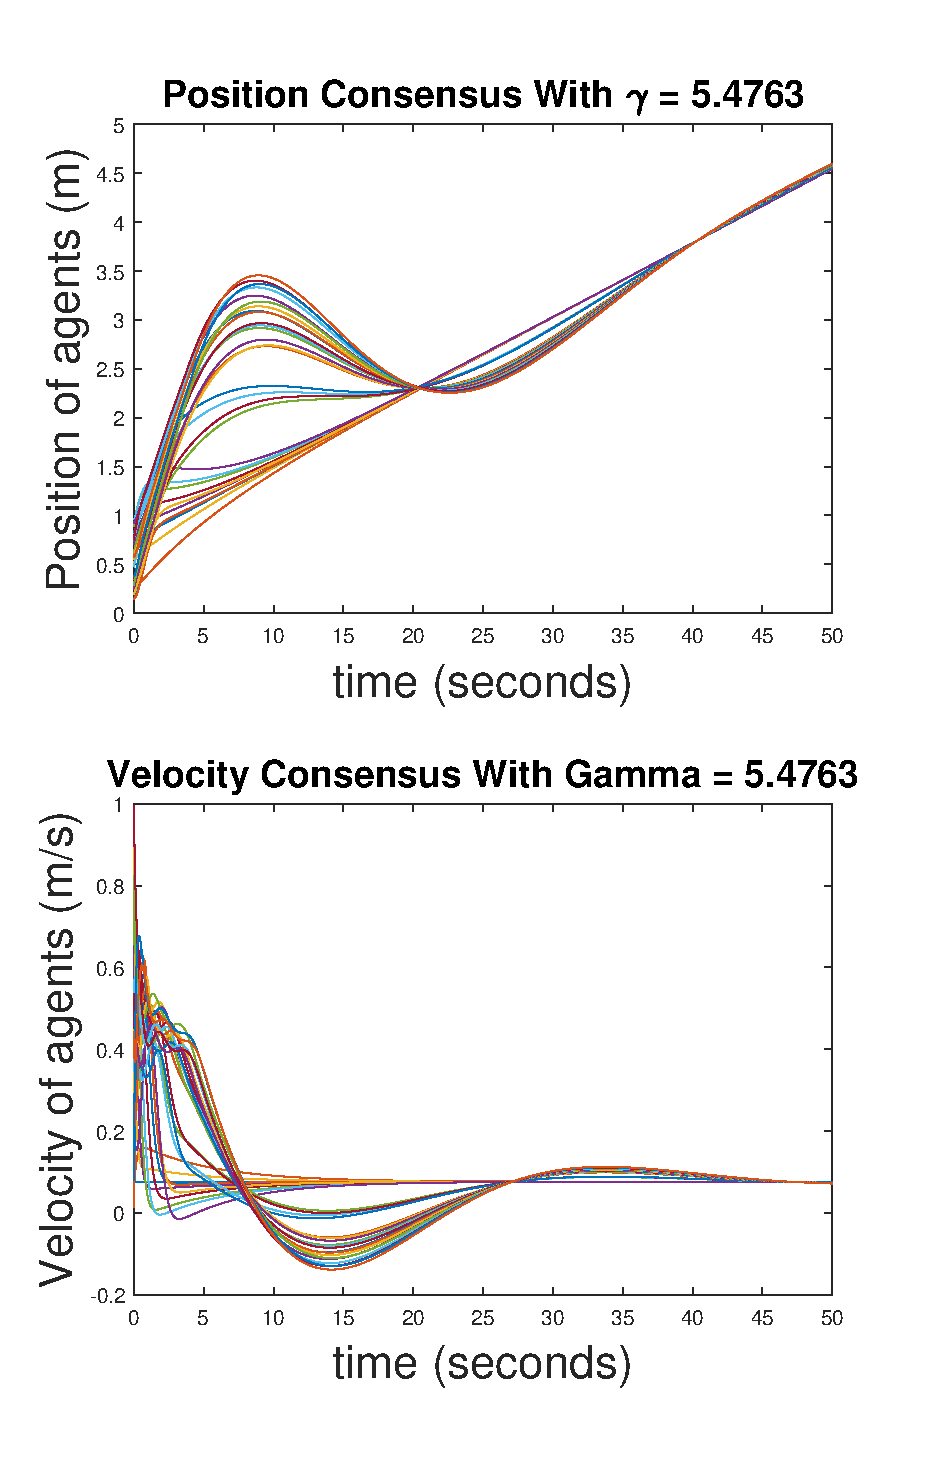
\includegraphics[width=0.75\textwidth,keepaspectratio]{2_Images/2.4.1_Position_Velocity_Combined_Sufficient_Gamma.eps}
\caption{Position and velocity consensus in the presence of two reverse edges, where $x_1<x_2=y_1<y_2$.}
\label{Case2bconsensus}
\end{figure}

\begin{figure}[ht!]
\centering
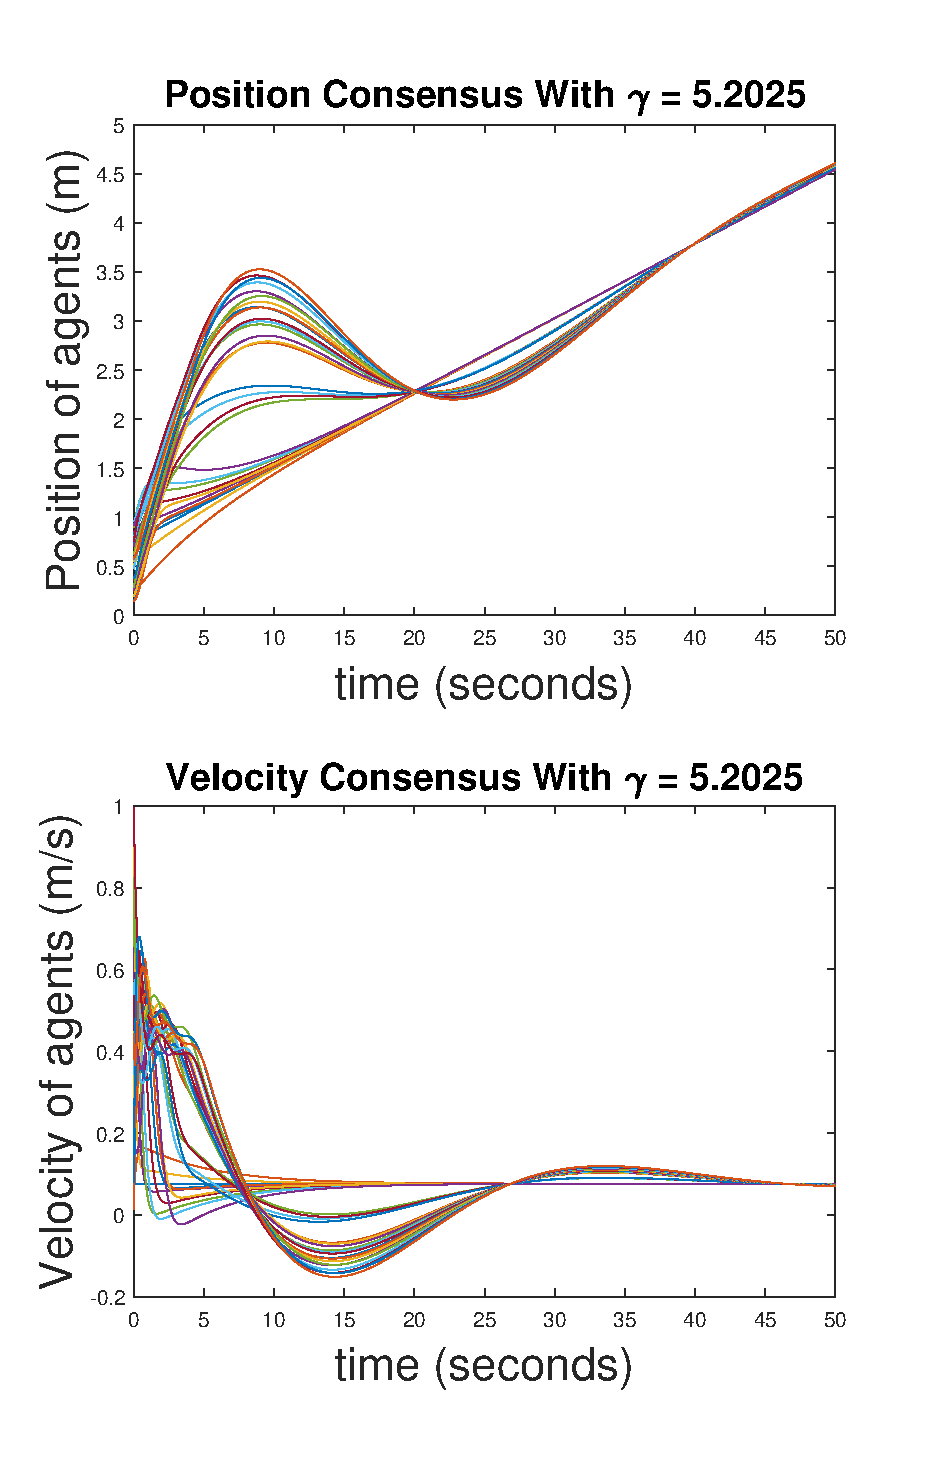
\includegraphics[width=0.75\textwidth,keepaspectratio]{2_Images/2.4.1_Position_Velocity_Combined_Below_Sufficient_Gamma.eps}
\caption{Position and velocity responses for a velocity coupling parameter slightly below the calculated sufficient value.}
\label{Case2bconsensus_below_calculated_gamma}
\end{figure}

\begin{figure}[ht!]
\centering
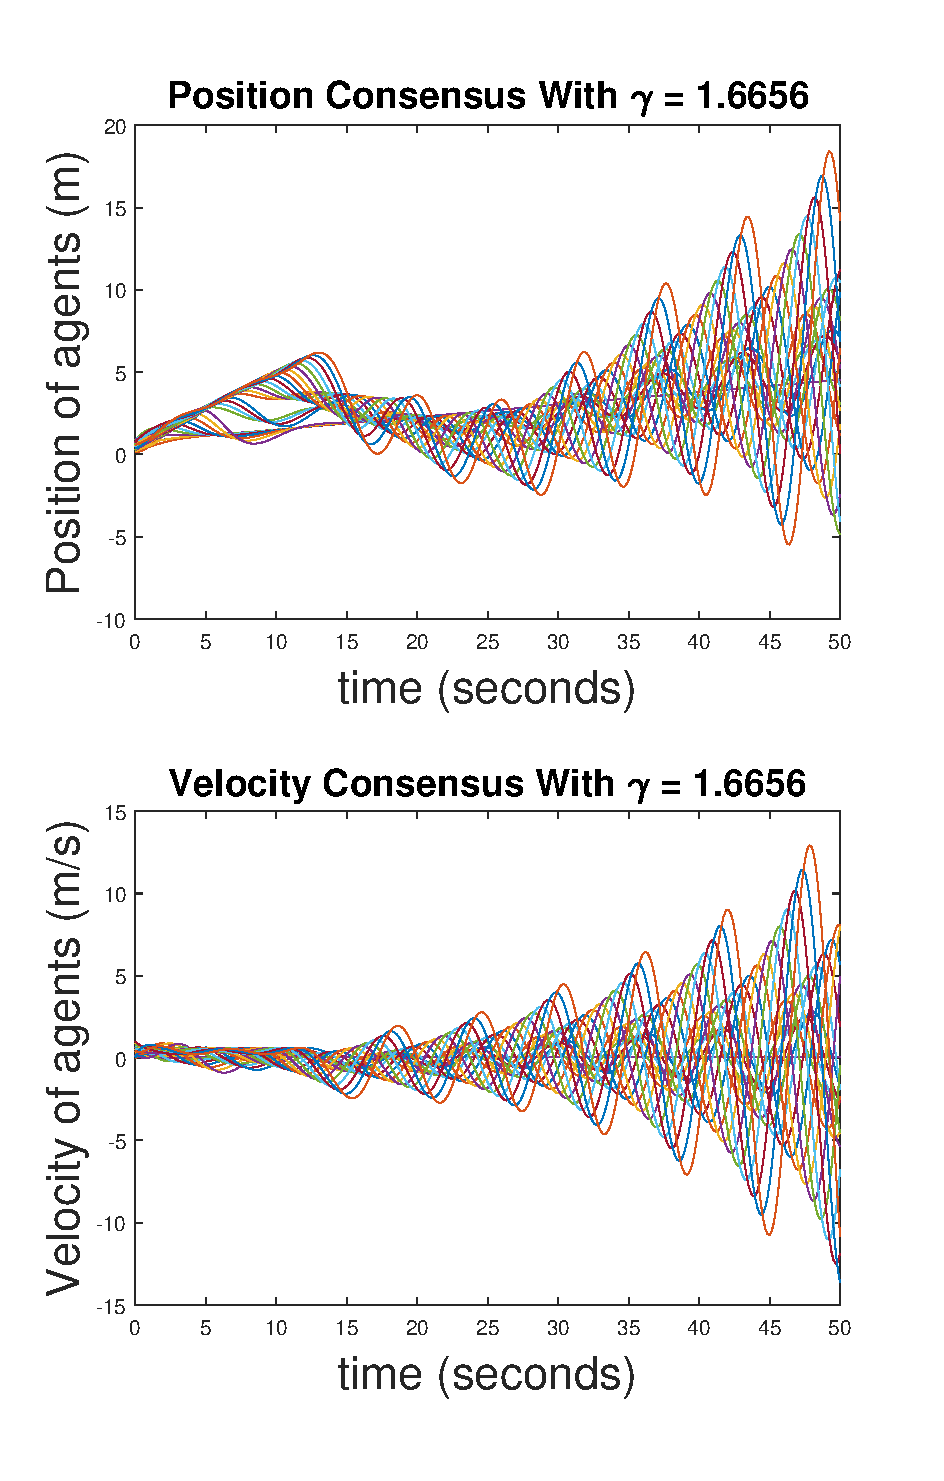
\includegraphics[width=0.75\textwidth,keepaspectratio]{2_Images/2.4.1_Position_Velocity_Combined_Below_Threshold_Gamma.eps}
\caption{Breakdown of position and velocity consensus when the velocity coupling parameter is below the stability threshold.}
\label{Case2bconsensus_Below_Threshold}
\end{figure}

\subsection{Second-order consensus in directed topology of Case~\ref{Case3}(c)}
%	Consider the network as shown in Fig.~\ref{Case3}, with $N=30$, $x_1=10$, $x_2=15$, $y_1=20$ and $y_2=25$. Applying Theorems \ref{theo9} and \ref{theo11}, for consensus of double integrators, the real solution obtained is equal to 0.0275 and corresponding $\gamma=6.0339$. As we can see from Figure~\ref{Case3cconsensus}, the consensus in position is achieved with the given $\gamma$ value. Positional consensus establishes the fact that consensus in velocity has also been achieved, since otherwise positional consensus would have been untenable. Hence, positional consensus is sufficient to conclude about consensus in all the states of the multi-agent system in this case. However, for completeness, the velocity consensus plot has also been included in the figure.

% The gamma value calculated above is as per sufficiency condition. However, if the gamma is calculated as per necessary and sufficient condition given in \ref{eq:ch_TRE_yuexactbound}, the value of $\gamma=2.3216$. To show the consensus breakdown, a simulation with $\gamma=0.95*2.3216=2.2055$ is shown in Fig \ref{Case3cconsensusBreakdown}.

To validate the theoretical bounds established in Theorem~\ref{theo9} and Theorem~\ref{theo11}, we consider the directed chain network depicted in Fig.~\ref{Case3} with $N = 30$ second-order agents. The reverse feedback edges are configured with coordinates $x_1 = 10$, $x_2 = 15$, $y_1 = 20$, and $y_2 = 25$. 

This network realization corresponds to Case~3(c) (partially overlapping feedback loops of equal cycle length), where:
\begin{equation}
    l_1 = y_1 - x_1 = 10, \quad l_2 = y_2 - x_2 = 10.
\end{equation}
Substituting $l_1 = l_2 = 10$ into the characteristic polynomial defined in Theorem~\ref{theo9} yields:
\begin{equation}
    s^{12} + 2s^{11} + s^{10} - 2s = 1.
    \label{eq:sim_char_poly}
\end{equation}
By Lemma~\ref{Lemma:ch_TRE_poly1}, \eqref{eq:sim_char_poly} possesses a unique real root in $(0, 1)$, numerically evaluated as $s_1 = 0.0275$. The corresponding dominant convergence rate is $\mathfrak{Re}(\lambda_2(\mathcal{L})) = 1 - s_1 = 0.9725$. Applying the sufficiency condition formulated in Theorem~\ref{theo11}, the required velocity coupling gain evaluates to:
\begin{equation}
    \gamma_{\text{suff}} = \frac{1}{\sqrt{1 - s_1}} = \frac{1}{\sqrt{0.9725}} \approx 6.0339.
\end{equation}

As demonstrated in Fig.~\ref{Case3cconsensus}, choosing $\gamma = 6.0339$ guarantees asymptotic agreement among the agent states. Positional consensus $\lim_{t \to \infty} \|p_i(t) - p_j(t)\| = 0$ inherently guarantees velocity synchronization $\lim_{t \to \infty} \|v_i(t) - v_j(t)\| = 0$, as double-integrator dynamics ($\dot{p}_i = v_i$) render persistent positional alignment untenable in the presence of velocity divergence. Consequently, achieving positional consensus is mathematically sufficient to certify full-state consensus; nevertheless, the velocity profile is provided in Fig.~\ref{Case3cconsensus} for completeness.

While the value $\gamma = 6.0339$ satisfies the sufficiency condition of Theorem~\ref{theo11}, the exact stability boundary is dictated by the necessary and sufficient condition given in \eqref{eq:ch_TRE_yuexactbound}:
\begin{equation}
    \gamma_{\text{exact}} = \max_{i \in \{2, \dots, N\}} \frac{\mathfrak{Im}(\lambda_i(\mathcal{L}))}{|\lambda_i(\mathcal{L})|} \sqrt{\frac{1}{\mathfrak{Re}(\lambda_i(\mathcal{L}))}} = 2.3216.
\end{equation}
To demonstrate the sharpness of this theoretical boundary and illustrate consensus breakdown, a comparative simulation is executed with a sub-critical velocity coupling gain set slightly below the threshold:
\begin{equation}
    \gamma = 0.95 \times \gamma_{\text{exact}} = 0.95 \times 2.3216 = 2.2055.
\end{equation}
The resulting closed-loop response is depicted in Fig.~\ref{Case3cconsensusBreakdown}, showing dynamic divergence and sustained growing oscillations across the network.

	\begin{figure}[ht!]
    \centering
		%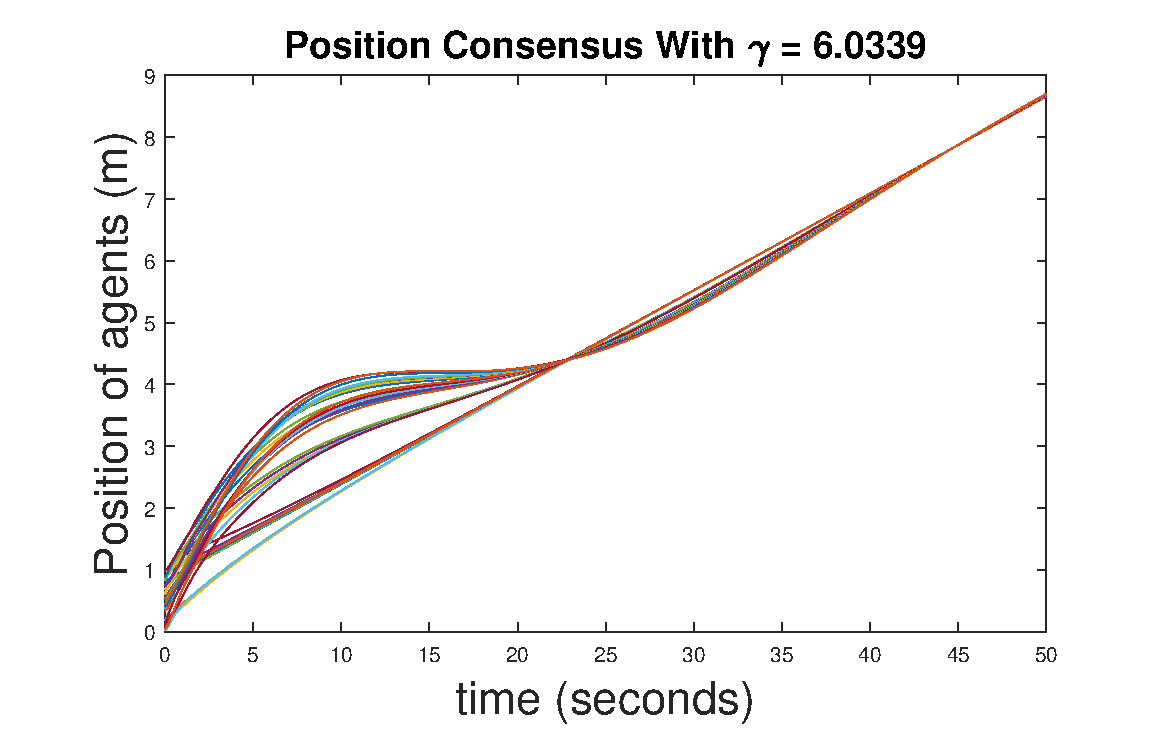
\includegraphics[width=0.75\textwidth,keepaspectratio]{2_Images/position_plot_for_theis.eps}
        %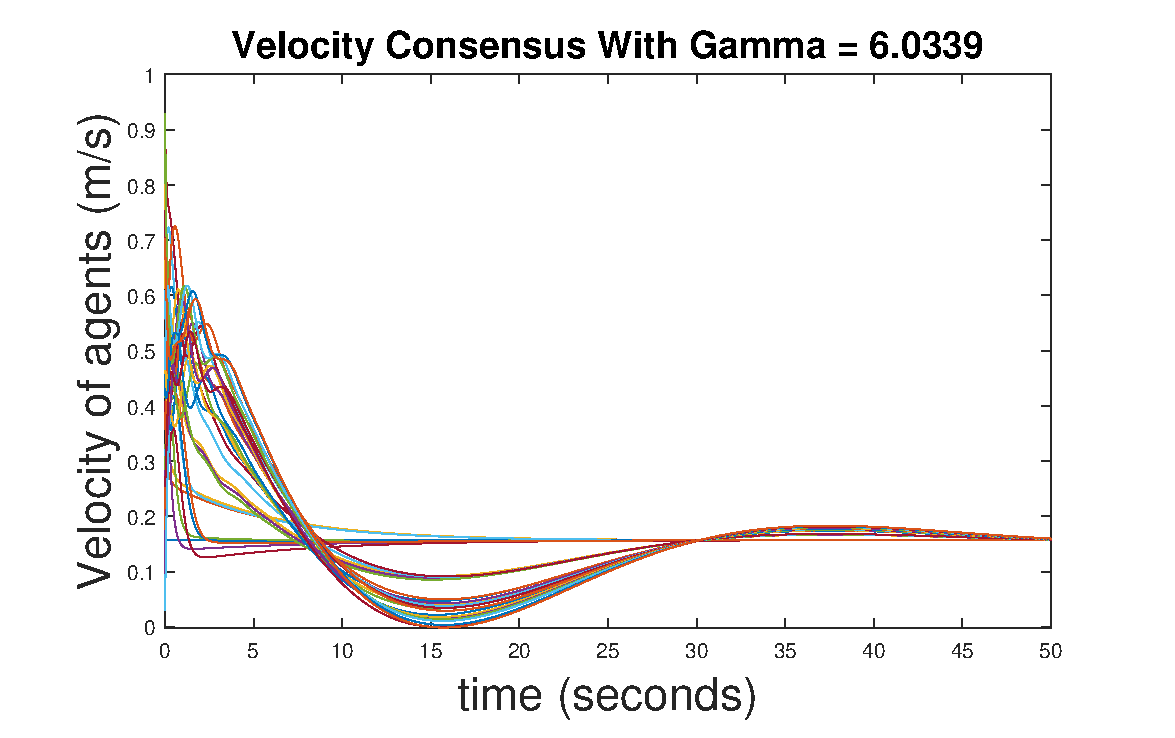
\includegraphics[width=0.75\textwidth,keepaspectratio]{2_Images/velocity_plot_for_theis.eps}
        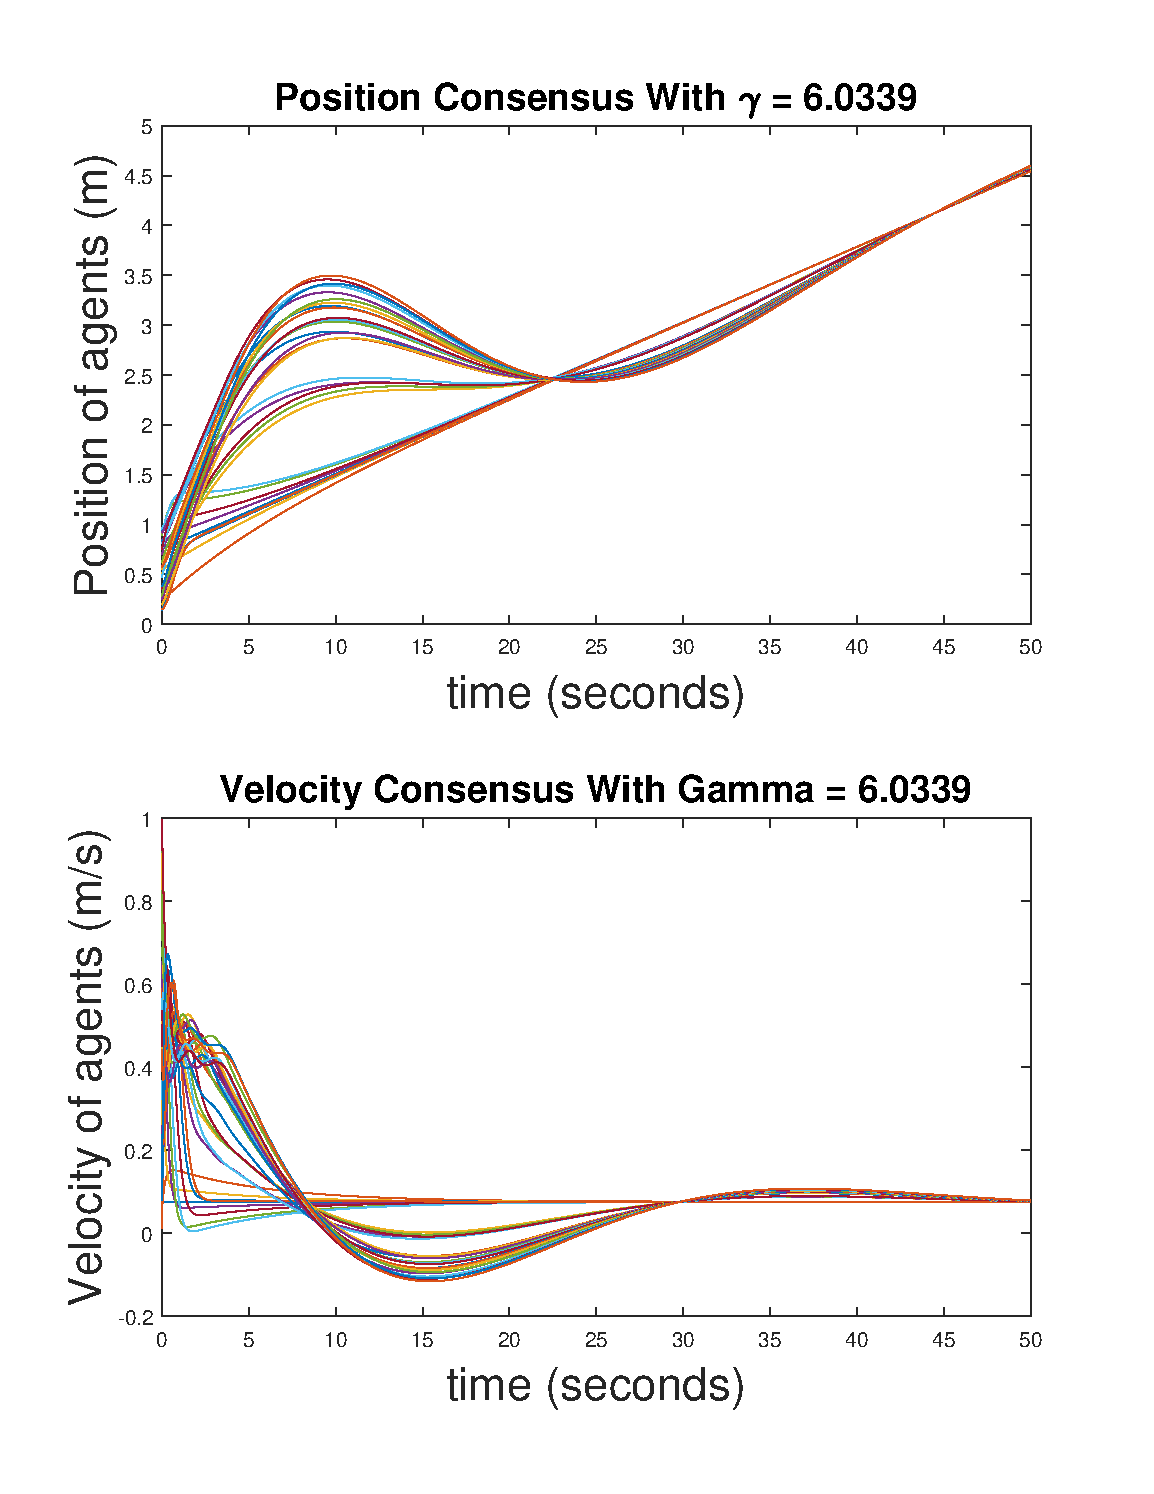
\includegraphics[width=0.75\textwidth,keepaspectratio]{2_Images/New_Stable.eps}
		\caption{Position and Velocity consensus in presence of two reverse edges where $x_1<x_2<y_1<y_2$}
		\label{Case3cconsensus}
	\end{figure}
    \begin{figure}[ht!]
    \centering
		%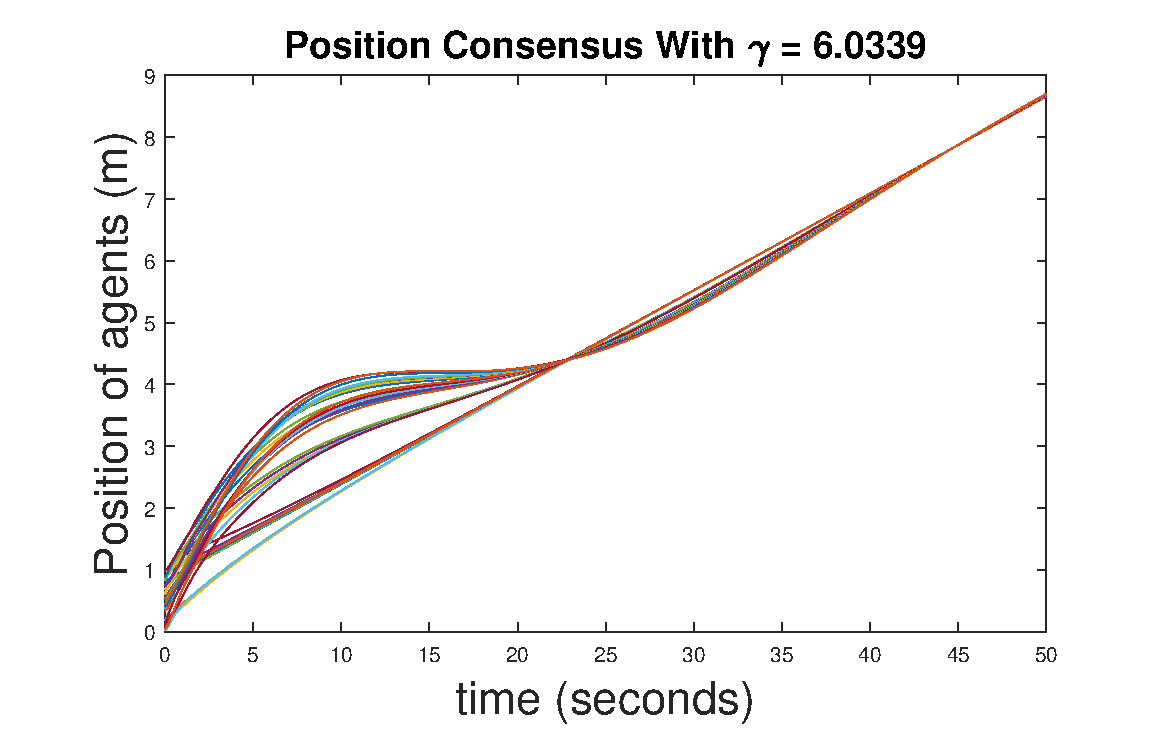
\includegraphics[width=0.75\textwidth,keepaspectratio]{2_Images/position_plot_for_theis.eps}
        %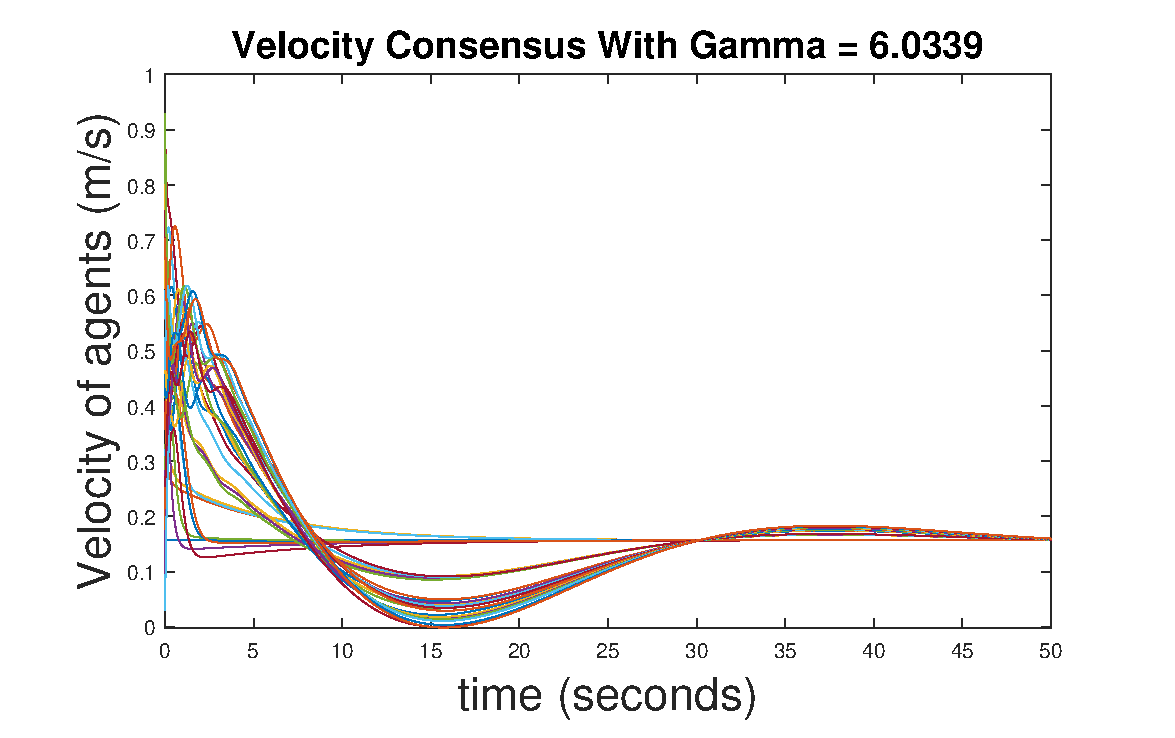
\includegraphics[width=0.75\textwidth,keepaspectratio]{2_Images/velocity_plot_for_theis.eps}
        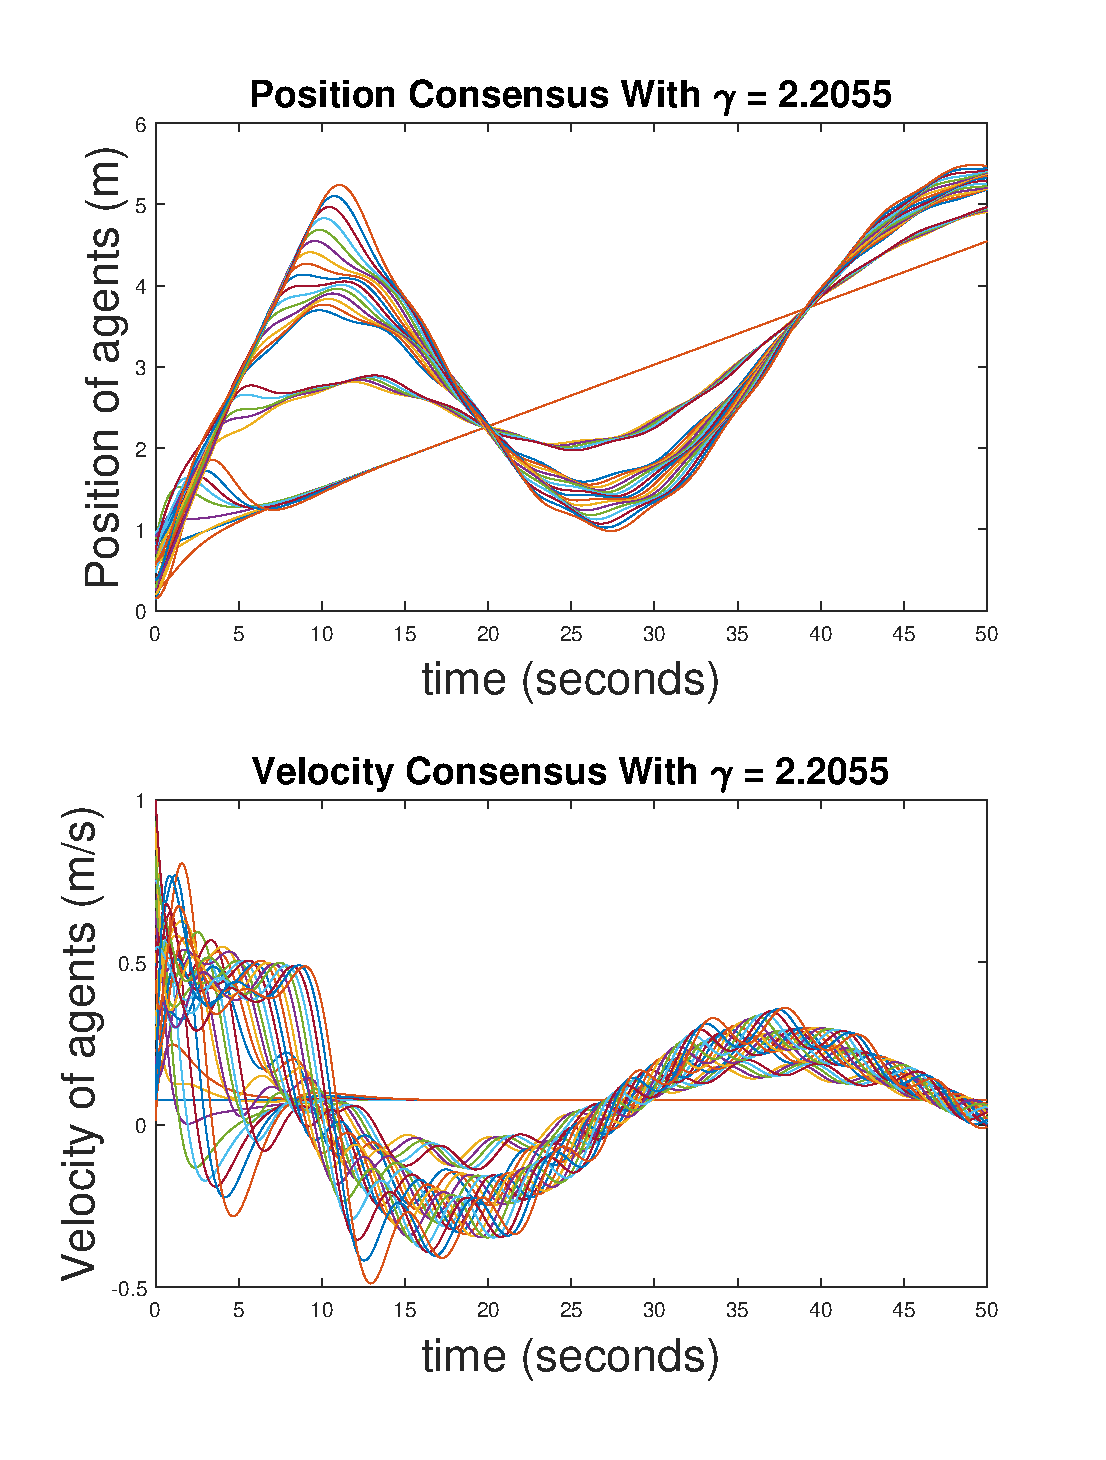
\includegraphics[width=0.75\textwidth,keepaspectratio]{2_Images/New_Unstable.eps}
		\caption{Consensus Breakdown in presence of two reverse edges where $x_1<x_2<y_1<y_2$}
		\label{Case3cconsensusBreakdown}
	\end{figure}

\section{Summary}\label{sec:ch_TRE_Summary}
In this chapter, we investigated the spectral impact of introducing dual reverse feedback edges across a directed chain network of double-integrator agents. The main findings and contributions of this chapter are summarized as follows:
\begin{itemize}
    \item \textbf{Exhaustive Topological Spectral Analysis:} We derived exact univariate characteristic polynomial equations across all six possible dual-loop spatial configurations (Cases 1–6) without imposing restrictive cycle-length or node-positioning assumptions.
    \item \textbf{Velocity Coupling Boundaries:} We proved that the dominant Laplacian eigenvalue $\lambda_2 = 1 - s_1$ is strictly governed by the unique real solution $s_1 \in (0,1)$ of the corresponding transformed polynomial. This real root dictates the exact non-negotiable lower bound on the velocity coupling gain ($\gamma \ge 1/\sqrt{1 - s_1}$) required to prevent dynamic divergence.
    \item \textbf{The Root-Node Loop Structural Singularity:} We formally established the Eigenvalue Shift Theorem (Theorem \ref{theo12}), proving that a loop of range $\ell$ alters $\ell+1$ eigenvalues when the root node is exterior ($x_1 > 1$), but affects only $\ell$ non-zero eigenvalues when the root node participates in loop formation ($x_1 = 1$).
    \item \textbf{Inherent Limitation of Global Polynomial Methods:} We proved that when $x_1 = 1$, standard polynomial methods collapse entirely, yielding the uninformative trivial solution $s_1 = 1 \implies \lambda_2 = 0$. This occurs because embedding the leader node in a feedback loop destroys its zero in-degree property ($d_{\text{in}, 1} > 0$), collapsing the leader-follower hierarchy and transforming all cycle nodes into co-equal root nodes.
\end{itemize}

The theoretical collapse of consensus, identified in Section 2.4, reveals a critical design issue for physical multi-agent networks: if an operational system has a fixed, predesigned velocity coupling gain $\gamma$ (or if a feedback loop enters the leader node $x_1 = 1$), traditional global spectrum re-computation fails to guarantee stability. 

To overcome these fundamental limitations, without requiring global network retuning or complete spectral evaluation of the Laplacian, Chapter \ref{ch:Guaranteed_Consensus} formulates a \textbf{decentralized, localized edge-weight perturbation framework}. By leveraging Gershgorin's Disc Theorem, sub-block shifts, local Node-Scaling, Edge-Scaling, and Root-Locus based tuning algorithms are synthesized to restore second-order consensus and resolve the root-node loop singularity under fixed coupling constraints.